\documentclass[journal]{IEEEtran}

\usepackage[utf8]{inputenc}
\usepackage{graphicx}
\usepackage{verbatim}
\usepackage{color}
\usepackage{xcolor}
\usepackage{xspace}
\usepackage [sorting=none] {biblatex}
\bibliography {rady20nofree}

\graphicspath{{figs/}}

\newcommand{\fsk}          {FSK 868 MHz}
\newcommand{\oqpsk}        {O-QPSK 2.4GHz}
\newcommand{\ofdm}         {OFDM 868 MHz}

\newcommand{\todo}[1]      {\textbf{\textcolor{red}{[TODO] #1}}}
\newcommand{\lorem}        {\textcolor{green}{Lorem ipsum dolor sit amet, consectetur adipiscing elit, sed do eiusmod tempor incididunt ut labore et dolore magna aliqua. Ut enim ad minim veniam, quis nostrud exercitation ullamco laboris nisi ut aliquip ex ea commodo consequat. Duis aute irure dolor in reprehenderit in voluptate velit esse cillum dolore eu fugiat nulla pariatur. Excepteur sint occaecat cupidatat non proident, sunt in culpa qui officia deserunt mollit anim id est laborum.}}
\newcommand{\mina}[1]      {\textbf{\textcolor{blue}{[Mina] #1}}}
\newcommand{\quentin}[1]   {\textbf{\textcolor{blue}{[Quentin] #1}}}
\newcommand{\dominique}[1] {\textbf{\textcolor{blue}{[Dominique] #1}}}
\newcommand{\thomas}[1]    {\textbf{\textcolor{blue}{[Thomas] #1}}}

\begin{document}

\title{No Free Lunch: 6TiSCH Performance\\on Different Modulations}

\author{
    \IEEEauthorblockN{
        Mina~Rady\IEEEauthorrefmark{1}\IEEEauthorrefmark{2},
        Quentin~Lampin\IEEEauthorrefmark{1},
        Dominique~Barthel\IEEEauthorrefmark{1},
        Thomas~Watteyne\IEEEauthorrefmark{2}
    }\\
    \IEEEauthorblockA{
        \IEEEauthorrefmark{1}~Orange Labs, Meylan, France
    }\\
    \IEEEauthorblockA{
        \IEEEauthorrefmark{2}~EVA team, Inria, Paris, France
    }
    \thanks{Corresponding author: Mina~Rady (email: {\tt poipoi})}https://www.overleaf.com/project/5e99476cb8ddc80001a31015
}

\maketitle

\begin{abstract}
   \lorem
   \lorem
   \lorem
\end{abstract}

\tableofcontents

%==============================================================================
\section{Introduction}
\label{sec:introduction}

% intro low-power wireless

Low-power wireless communications have undergirded the fourth industrial revolution by means of enabling pervasive machine-to-machine communications, otherwise known as the Internet of Things.
The range of applications of such technologies vary from smart-building monitoring \cite{munoz18overview}, \cite{kazmi14review}, environmental monitoring \cite{munoz18evaluationa}, precision agriculture \cite{watteyne16peach}, utility meter remote reading \cite{sum17experimental}, localization of expensive equipment \cite{tanakademo}, smart grid monitoring \cite{fadel15survey} and industrial equipment monitoring for predictive maintenance \cite{civerchia17industrial}.
Therefore, the financial value provided by such technology pour into a large array of economic sectors.
A plethora of radio technologies have been introduced to serve the IoT communications demands in different contexts and with different features.
For example, LoRa, a family of long range modulations, introduce a low-bitrate high link-budget modulations for battery powered devices.
LoRaWAN architectures are star-based topologies and they operate and Aloha-based Medium Access Control (MAC).
Therefore, it is non-deterministic and the network performance depends heavily on the level of contention in the medium \cite{adelantado17understandinga}.

% popular PHY layers
% \lorem IEEE802.15.4
Another major player in the IoT communications market is the set of technologies under the IEEE802.15.4 family of standards which were conceived in 2003 yet extended in several amendments since then. \cite{11ieee}
The  IEEE802.15.4e amendment defines a MAC sublayer that follows the Time-Slotted Channel Hopping (TSCH) paradigm for low-rate wireless personal area networks \cite{12ieeea}.
In contrast to a non-deterministic protocol as LoRaWAN, the TSCH paradigm is capable of providing wire-like reliability due to the strict allocation of time and frequency resources in the network based on a hashing scheme of IPv6 addresses of the nodes \cite{t.chang206tisch}.
By means of this allocation, transmissions occur, mostly, in dedicated combinations of time-slots and channels (also known as cells).
This allows the mitigation of the side-effects of contention, although it does not completely remove them because a minor subset of network management transactions have to take place still in "shared" cells, where contention is still possible.

The IEEE802.15.4g amendment defines physical layer specifications for low-data-rate, wireless, smart metering utility networks \cite{12ieee}.
This amendment was rolled into the 2016 edition of the IEEE802.15.4 standard, which includes the following three families of multi-rate and multi-regional (MR) modulations: 1) Frequency Shift Keying (MR-FSK), 2) offset quadrature phase-shift keying (MR-O-QPSK), and 3) orthogonal frequency division multiplexing (MR-OFDM).
Furthermore, several frequency bands are defined as part of the standard as common communication ``channels" in the license-free bands.
While the license-free frequency bands may vary depending national regulations, they are usually split into two main categories: the 2.4 GHz band and the sub-GHz band. 
The 2.4 GHz band is usually characterized by lower link-budget and shorter range than the sub-GHz band (due to the higher frequency). 
This makes it sufficient for small home-area networks, yet it makes it highly susceptible to interference from common technologies in the same band such as WiFi \cite{tuset-peiro19experimental}
The sub-GHz band is usually characterized by higher link budget and longer range than the 2.4 GHz band. 
This makes it suitable for challenging deployments such as kilometer-scale links in rural areas or complex indoor environments \cite{sotokmscale}.
The modulations in this amendment support a wide range of bitrates as low as 25 kbps and as high as 800 kbps (in the European ISM bands)

% capabilites of recent chips

% \lorem nRF52840, CC2538, CC2650
Several radio chips and System-on-Chip (SoC) products have been increasingly introduced to the market in compliance with the IEEE802.15.4g standard. 
As manufacturing technology advanced, chips started to offer multiple modulations and even multiple frequency bands depending on how their registers are configured by program running on the micro-processor.
Common examples of these systems are CC2538 \cite{12cc2538} and CC2650 \cite{15cc2650} SoCs by Texas Instruments and nRF52840 \cite{19nrf52840} by Nordic Semiconductor. 
They are built around a 32-bit ARM cortex microprocessor with electrical features supporting low-power performance.
Their radio-chip design allows the choice of modulation and frequency band by the executing program among any of the options under the IEEE802.15.4g standard. 
The example host board used for the experiments in this paper is the OpenMote-B which features a 2.4 GHz antenna and a sub-GHz antenna \cite{tusetopenmote}.

% goal
The IPv6 Time Slotted Channel Hopping (6TiSCH) protocol stack has been  standardized by the Internet Engineering Task Force (IETF).
The MAC layer of 6TiSCH is the IEEE802.15.4e standard allowing industrial-grade reliability.
The PHY layer of 6TiSCH is the IEEE802.15.4 standard allowing a wide variety of selection among the aforementioned modulations supported by the standard.
Most researched 6TiSCH implementations rely almost canonically on O-QPSK PHY layer in the 2.4 GHz band, as demonstrated by \cite{j.munoz18problem} and \cite{brachmann19ieee}.
This limits the stack performance by the limitations of the short range \oqpsk  radio and discards potential advantages of other modulations such as higher link-budget --enabling km-scale connectivity, or very high bit-rates up to 800 kbps --enabling lower radio duty cycles.
Furthermore, there is no evidence on how the change of the PHY layer could impact the performance of the 6TiSCH network as a whole. 

Therefore, he goal of this paper is to compare the system-level performance of the 6TiSCH stack on top of three PHY layers among the IEEE802.15.4g standard that are of complementary characteristics: 
     1) A high-frequency, high bit-rate option: O-QPSK in the 2.4 GHz band, offering a nominal bitrate of 250 kbps,
     2) A low bit-rate, low frequency option: FSK option 1 in the 868 MHz band, offering nominal bit-rate of 50 kbps, and 
     3) A high bit-rate, low frequency option: OFDM option 1  in the 868 MHz band, with Modulation and Cosing Scheme (MCS) 3, offering a nominal bit-rate of 800 kbps. 


%==============================================================================
\section{Related Work}
\label{sec:related_work}

% Problem statement

While active research proposed various enhancements in 6TiSCH  for more wire-like reliability with low power consumption, there is one assumption about 6TiSCH that remained constant for nearly two decades: it uses the IEEE802.15.4 (2003) O-QPSK modulation in 2.4 GHz band in as its PHY layer. 
There is no doubt that \oqpsk may be sufficient in some applications, however the increasing demands for long range connectivity for several applications (such as environmental monitoring or wireless utility metering) can only be met by considering longer range radios for the 6TiSCH PHY layer.
A problem statement has been proposed in the Internet Engineering Task Force (IETF) detailing the theoretical challenges or side-effects of re-inventing the 6TiSCH PHY layer to include different or heterogeneous radios other than the canonical \oqpsk \cite{j.munoz18problem}. 
Although the protocol stack layers remain separate, it is reasonable to expect, in light of this problem statement, that a change in one layer might impact the end-to-end performance as a whole. 
Utilization of a different PHY layer means, for example, different energy consumption and link-costs which would change how links to neighbors are evaluated at layer 2 and how routes are calculated at layer 3.
It also means there is an expectation of more re-transmissions for high-frequency bands, more interference or collisions in shared cells for low-frequency bands.
Therefore, even though only the PHY layer is expected to change, a system level evaluation in line with the end-to-end argument in computer systems design \cite{saltzer84endtoend} is indispensable.
This is to evaluate the (potential) impact of such change on the network functions placed at the end of the communication pipe-line. 

% Related work is split into three main categories:
% networks for industrial iot
% 1- 6TiSCH performance evaluation
The related work is presented under three categories: 
    1) performance improvement and evaluation of the 6TiSCH protocol stack,
    2) performance evaluation of IEEE802.15.4g family of modulations, and
    3) hybrid radio utilization in the 6TiSCH stack. 
The remaining of this section will present each category and discuss its relevance to this paper.

\textit{1) Performance improvement and evaluation of the 6TiSCH protocol stack:} authors of \cite{sum17experimental} provide an experimental evaluation of IEEE802.15.4e Time Slotted Channel Hopping MAC based on IEEE802.15.4g radio.
The experiments report range and performance testing results in terms of PDR and PER in four situations: LOS conditions, NLOS conditions, tree topology in corridor setting and line topology across buildings.

Authors of \cite{yang18analysis} evaluate the performance of the full 6TiSCH stack on the OpenWSN reference architecture in terms of responsiveness to time critical event triggers.
They vary the number of active slots in an 11 slot-frame length and measure how packet end-to-end latency is affected withe the variance of active slots. 

Authors of \cite{theoleyre16experimental} evaluate the performance of the 6TiSCH stack with the deployment of traffic isolation mechanisms that allow reservation of dedicated slots for certain applications and reservation of shared slots for alarm events.
They report the end-to-end latency and PDR under various schedule management strategies, including using uniformly distributed shared cells instead of contiguous (adjacent) shared cells in the slot-frame.

Authors of \cite{teleshermeto18reactions} execute a performance evaluation of the 6TiSCH protocol stack in an indoor environment with a focus on the stability of the stack performance.
They report the end-to-end reliability and number of parent changes as the network is converging.
They also propose a stable link quality metric and a simplified method for schedule inconsistency management. 

Finally, the research in \cite{benyaala16performance}, evaluates the performance of 6TiSCH stack in co-located networks.
It considers both cases where the coexisting 6TiSCH networks are either  synchronized or unsynchronized.

There is one common factor among all this work: the chosen PHY layer remains unchanged and therefore the impact of changing the PHY layer is not considered. 
They are all based on the IEEE802.15.4 (2003) \oqpsk , except \cite{sum17experimental} which use MR-FSK throughout the experiments. 

% one phy layer
% 2- 802.15.4g evaluation:

\textit{IEEE802.15.4g performance evaluation:} this category  demonstrates the related  work attempting to evaluate different IEEE802.15.4g PHY layers in one way or another.
Research in \cite{kojima15system} examines the impact of interference between two modulations of IEEE802.15.4g, namely: MR-FSK mode 2 and MR-OFDM option 4 MCS 3. 
Authors deploy IEEE802.15.4e MAC with multihop capability on top of each PHY layer and measure the impact of the interference between two networks, each running one PHY.
Results are reported in terms of the degradation of throughput of each network in the presence of the other interfering network.

The research in \cite{munoz18overview} runs experimental campaigns for comparative performance evaluations of two PHY layers for smart building applications: IEEE802.15.4 (2003) \oqpsk and IEEE802.15.4g MR-OFDM. 
Although \oqpsk offers a nominal bitrate of 250 kbps, the experimental results demonstrate surprising range-test performance of MR-OFDM compared to \oqpsk even at bit-rates up to 800 kbps in the case of OFDM Option 1 MCS 3. 
Furthermore, the paper shows that although \oqpsk consumes less power in general than \ofdm, it can lead to overall more power consumption for a successful transmission if the power consumed in re-transmissions is taken into account..  
The research in \cite{munoz18evaluationa} is the state of the art in the performance evaluation of the totality of IEEE802.15.4g modulations.
Authors perform exhaustive  range-testing campaigns of the 31 modulations in four scenarios that are considered the most prevalent in outdoor applications: line of sight, smart agriculture, urban canyon, and smart metering. 
Results of the range-tests are reported in terms of PDR measurements, throughput, and electric charge consumption.
Interesting findings show that OFDM in high bit-rates reaching up to 800 kbps can outperform 2-FSK PHY layer at low bit-rate of 50 kbps in range and reliability. 
This finding stresses caution against the assumption that lower bit rate modulations would be more reliable or longer in range because they are just low bit-rate \textit{per se}. 

Among all the work presented in this section, one common gap is present which is that the end-to-end performance of a full 6TiSCH stack remains unknown with the change of PHY layer. 
Therefore, it is still not clear how some system-level behaviours would be impacted such as the end-to-end  PDR, end-to-end latency, network formation time, and distribution of battery lifetime of the nodes in the network.  

% 3- hybrid radio utilization

\textit{Hybrid radio utilization in the 6TiSCH stack:}  research in \cite{brachmann19ieee} is the state of the art to integrate hybrid PHY layers within the 6TiSCH stack. 
First, authors perform range-testing measurements on multiple modulations, namely: 2-GFSK (at bit-rates 1.2, 8, 50, and 250 kbps), 4-GFSK (at bit-rate 1000 kbps), and \oqpsk (at bit-rate 250 kbps). 
Link quality evaluations are reported in terms of number of motes reached by each mote in the network and link symmetry. 
Second, authors choose two modulations in the sub-GHz band for integration in the 6TiSCH stack: 2-GFSK at bit-rate  1.2 kbps  for Enhanced Beacon (EB) transmissions in the minimal (shared) cells, and 4-GFSK at bit-rate 1000 kbps for data traffic. 
The reason authors make such a choice is to achieve a single-hop transmission for EB, using the slowest bit-rate modulation, in order to guarantee faster and more accurate synchronization in the network than multi-hop transmissions. 
Slot templates matching the chosen PHY layers are designed generally in accordance with IEEE802.15.4 standard and ported on Contiki-NG reference implementation of 6TiSCH. 
Finally, authors report performance of the multi-PHY network in terms of channel utilization and the distribution of synchronization accuracy in the network in comparison with the distribution of hop-count. 
Authors demonstrate that faster bit-rate of 4-GFSK at 1000 kbps for data packets diminishes the probability for collision and leads to less than 0.1\% channel utilization despite the increased re-transmissions.
At the same time, the slower bit-rate of 2-GFSK at 1.2 kbps for EB packets leads to 20x higher channel occupancy, at 2\% duty cycle (leading to violation of the license-free band regulation in many regions). 

This research paves the road for thorough investigation of multi-PHY integration in the 6TiSCH stack.
However, it explicitly assumes an inverse correlation between bit-rate and range.
While this could be true for the specific subset of modulations selected for evaluation, it is not in concordance with research results in \cite{munoz18overview} and \cite{munoz18evaluationa} , which demonstrate that a high bit-rate modulation such as OFDM 1 MCS 3 at 800 kbps can offer competitive performance compared to 2-FSK at 50 kbps in terms of range, reliability, let alone duty cycle. 
This is a significant observation because if long-range radio is needed for EB synchronization as \cite{brachmann19ieee} suggests, higher bit-rates are appreciated for EBs in order to minimize energy consumption and also collision probability since EBs are transmitted on shared cells. 
Furthermore, it still remains unclear whether there are any side-effects to the choice of one radio or another  on the end-to-end performance as a whole so that the costs and benefits of each PHY layer choice can be fully assessed.

%==============================================================================
\section{Contributions}
\label{sec:contributions}

This paper demonstrates that there are significant benefits of each of the radio options: \fsk, \ofdm, and \oqpsk, yet they all come at a certain cost of one kind or another.
Therefore, this demonstrates that there is no free lunch when it comes to the choice of PHY layer.
Precisely, the contributions of this paper are three-fold:

%
\begin{itemize}
    \item Augmenting OpenWSN reference architecture of the 6TiSCH protocol stack with support of 3 PHY layers, available as open source.
    \item Conducted exhaustive validation campaign of the end-to-end performance of the 6TiSCH stack on top of each PHY, on a testbed of 42 motes office environments.
    Results are reported in terms of end-to-end Key Perfromance Indicators (KPI) that are necessary reference metrics for performance evaluation and service-level agreements (SLAs)
    The KPIs are: 
        network formation time,
        end-to-end reliability,
        end-to-end latency, and
        estimated battery lifetime distribution in the network,
        and memory footprint.
    \item The paper shows the advantages and disadvantages of each PHY layer highlighting that not one PHY is the best across all KPIs.
\end{itemize}

As a result of the conducted evaluation campaigns, three lessons have been learned:

% lessons learned
\begin{itemize}
   \item \fsk\ PHY allows the most number of neighbors to be discovered by mote. 
    It leads to the fastest network formation time with the lowest latency and lowest network depth.Yet it shortens network battery lifetime \mina{note} due to high radio duty cycle. 
    It also risks neighbor table overflow in high density deployments.
   
   \item \oqpsk\  PHY allows that the least number of neighbors are discovered by a mote. 
   It leads to the slowest network formation time, highest network depth, and effectively the highest end-to-end latency. 
   It consumes the most packet buffer on average because of storage needed to re-transmissions, leading to a higher risk of packet-buffer overflow. 
   
   \item \ofdm\ PHY, allows the discovery of a surprisingly large number of neighbors close to \fsk, despite being the highest bit-rate in the three modulations. 
   It shows an intermediate network formation time, end-to-end latency, packet buffer occupancy and network depth.
   Yet despite its low duty cycle, it decreases the battery lifetime of the network by more than 65\% compared to \oqpsk.
\end{itemize}
  

The remainder of this article is organized as follows.
Section~\ref{sec:opentested} \todo{}.

%==============================================================================
\section{The OpenTestbed}
\label{sec:opentested}

% intro testbed, architecture
To perform the experiments for this paper, the OpenTestbed \cite{munoz19opentestbed} is found to be an appropriate choice for this context.
The OpnTestBed is built from off-the-shelf components without requiring any dedicated wiring infrastructure or back-end server, with an open access interface. 
Therefore, it can be re-used through remote access or even re-built locally, at low cost, to replicate the experiments in similar or different settings.  
The core components of the OpenTestBed are OpenMote B low power devices, Raspberry Pi single-board computers, and a glass dome container.
The general architecture is that each Raspberry Pi has four OpenMote-B devices attached to it through USB interface and it connects to an MQTT broker allowing bi-directional communication with the motes through remote access. 

% OpenMote and testbox

OpenMote-B a prototyping platform for the Industrial Internet of Things (IIoT) that is an enhancement to the OpenMote+ platform \cite{tusetopenmote}. 
As illustrated in in Fig. \ref{fig:testbox} in the left,  it features two radio chips: 
	1) CC2538 radio offering IEEE802.15.4 (2003) O-QPSK option at the 2.4 GHz band. This radio is part of the CC2538 SoC, and 
    2) AT86rf215 radio offering both 2.4 GHz and sub-GHz bands and the full suite of modulations options under the IEEE802.15.4g amendment (the three families of MR-FSK, MR-OFDM, and MR-O-QPSK). 
A 2.4 GHz antenna is connected to the CC2538 radio and a sub-GHz antenna is connected to the AT86rf215 radio.
This multi-PHY capability is the main enabler for the experiments required in this research. 
It is built aroudn the CC2538 ARM-cortex micropreocesor, which is the same used for industrial applications as in \cite{civerchia17industrial}.
The mote offers 32 KB of RAM and 512 KB Flash which were both sufficient for running the firmware of the 6TiSCH stack on top of OpenWSN Real Time Operating System (RTOS). 
Most importantly, it features two main debugging capabilities that enabled accurate timing configuration for the IEEE802.15.4e slot templates for several modulations:
1) Joint Test Action Group (JTAG) port, which enables on board-debugging of firmware behavior under the new developments the radio drivers and the MAC layer as explained in section \ref{sec:openwsn}, and 
2) Board expansion: which offered 8 pins which were indispensable for debugging. The pins were connected to a logic analyzer that allowed real-time view of the slot event triggers and synchronization accuracy.
Finally, motes are clustered such that each 4 motes were connected to a Raspberry Pi 3B + single-board computer, Fig. \ref{fig:testbox}, right.
Motes generate local statistics and information at run-time and forwards them via the serial port to the Raspberry PI. 
The Raspberry PI allows a bi-directional access to the motes via an MQTT broker and over a 5 GHz WiFi band so as not to interfere with the motes in case they use the 2.4 GHz band for their operation.
First, it allows remote boot-loading of firmware via the broker as explained in \cite{munoz19opentestbed}.
Second, it collects the serial output of the motes and forwards it to the  broker. 



\begin{figure}
	\centering
	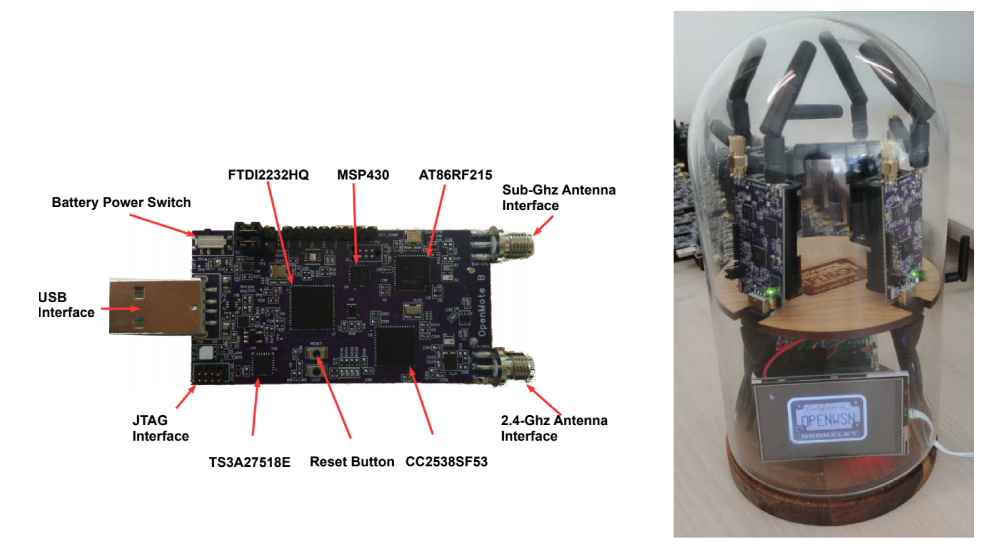
\includegraphics[width=0.90\columnwidth]{mote_ot}
	\caption{OpenMote B board (left) and The testbox containing four OpenMote B boards (right).}
    \label{fig:testbox}
\end{figure}

% 42-mote deployment

The test-bed is composed of 42 motes deployed across the floor of the EVA lab in Inria Paris as shown in Fig.\ref{fig:floorplan}.
Boxes are distributed to cover the floor, except in room A102 where a cluster of 18 motes are placed in the same room.
This distribution is distinct from the distribution used in \cite{brachmann19ieee} in that the nodes are distributed much less uniformly across the floor. 
In this distribution, we aim to introduce non-uniformity akin to that of a real world setting.
The reason is that in an industrial plant, such as in \cite{civerchia17industrial}, sensors are clustered around the locations of machines or production lines where sensor readings are needed for their predictive maintenance.
For example, the authors of \cite{civerchia17industrial} deploy clusters of sensors around the heavy ashes water pump, seawater pumps, and evaporators. 
The size of clusters varied from 3 wireless sensors per cluster up to 19 wireless sensors per cluster (in the case of the evaporator equipment consisting of multiple pumps). 



\begin{figure}
	\centering
	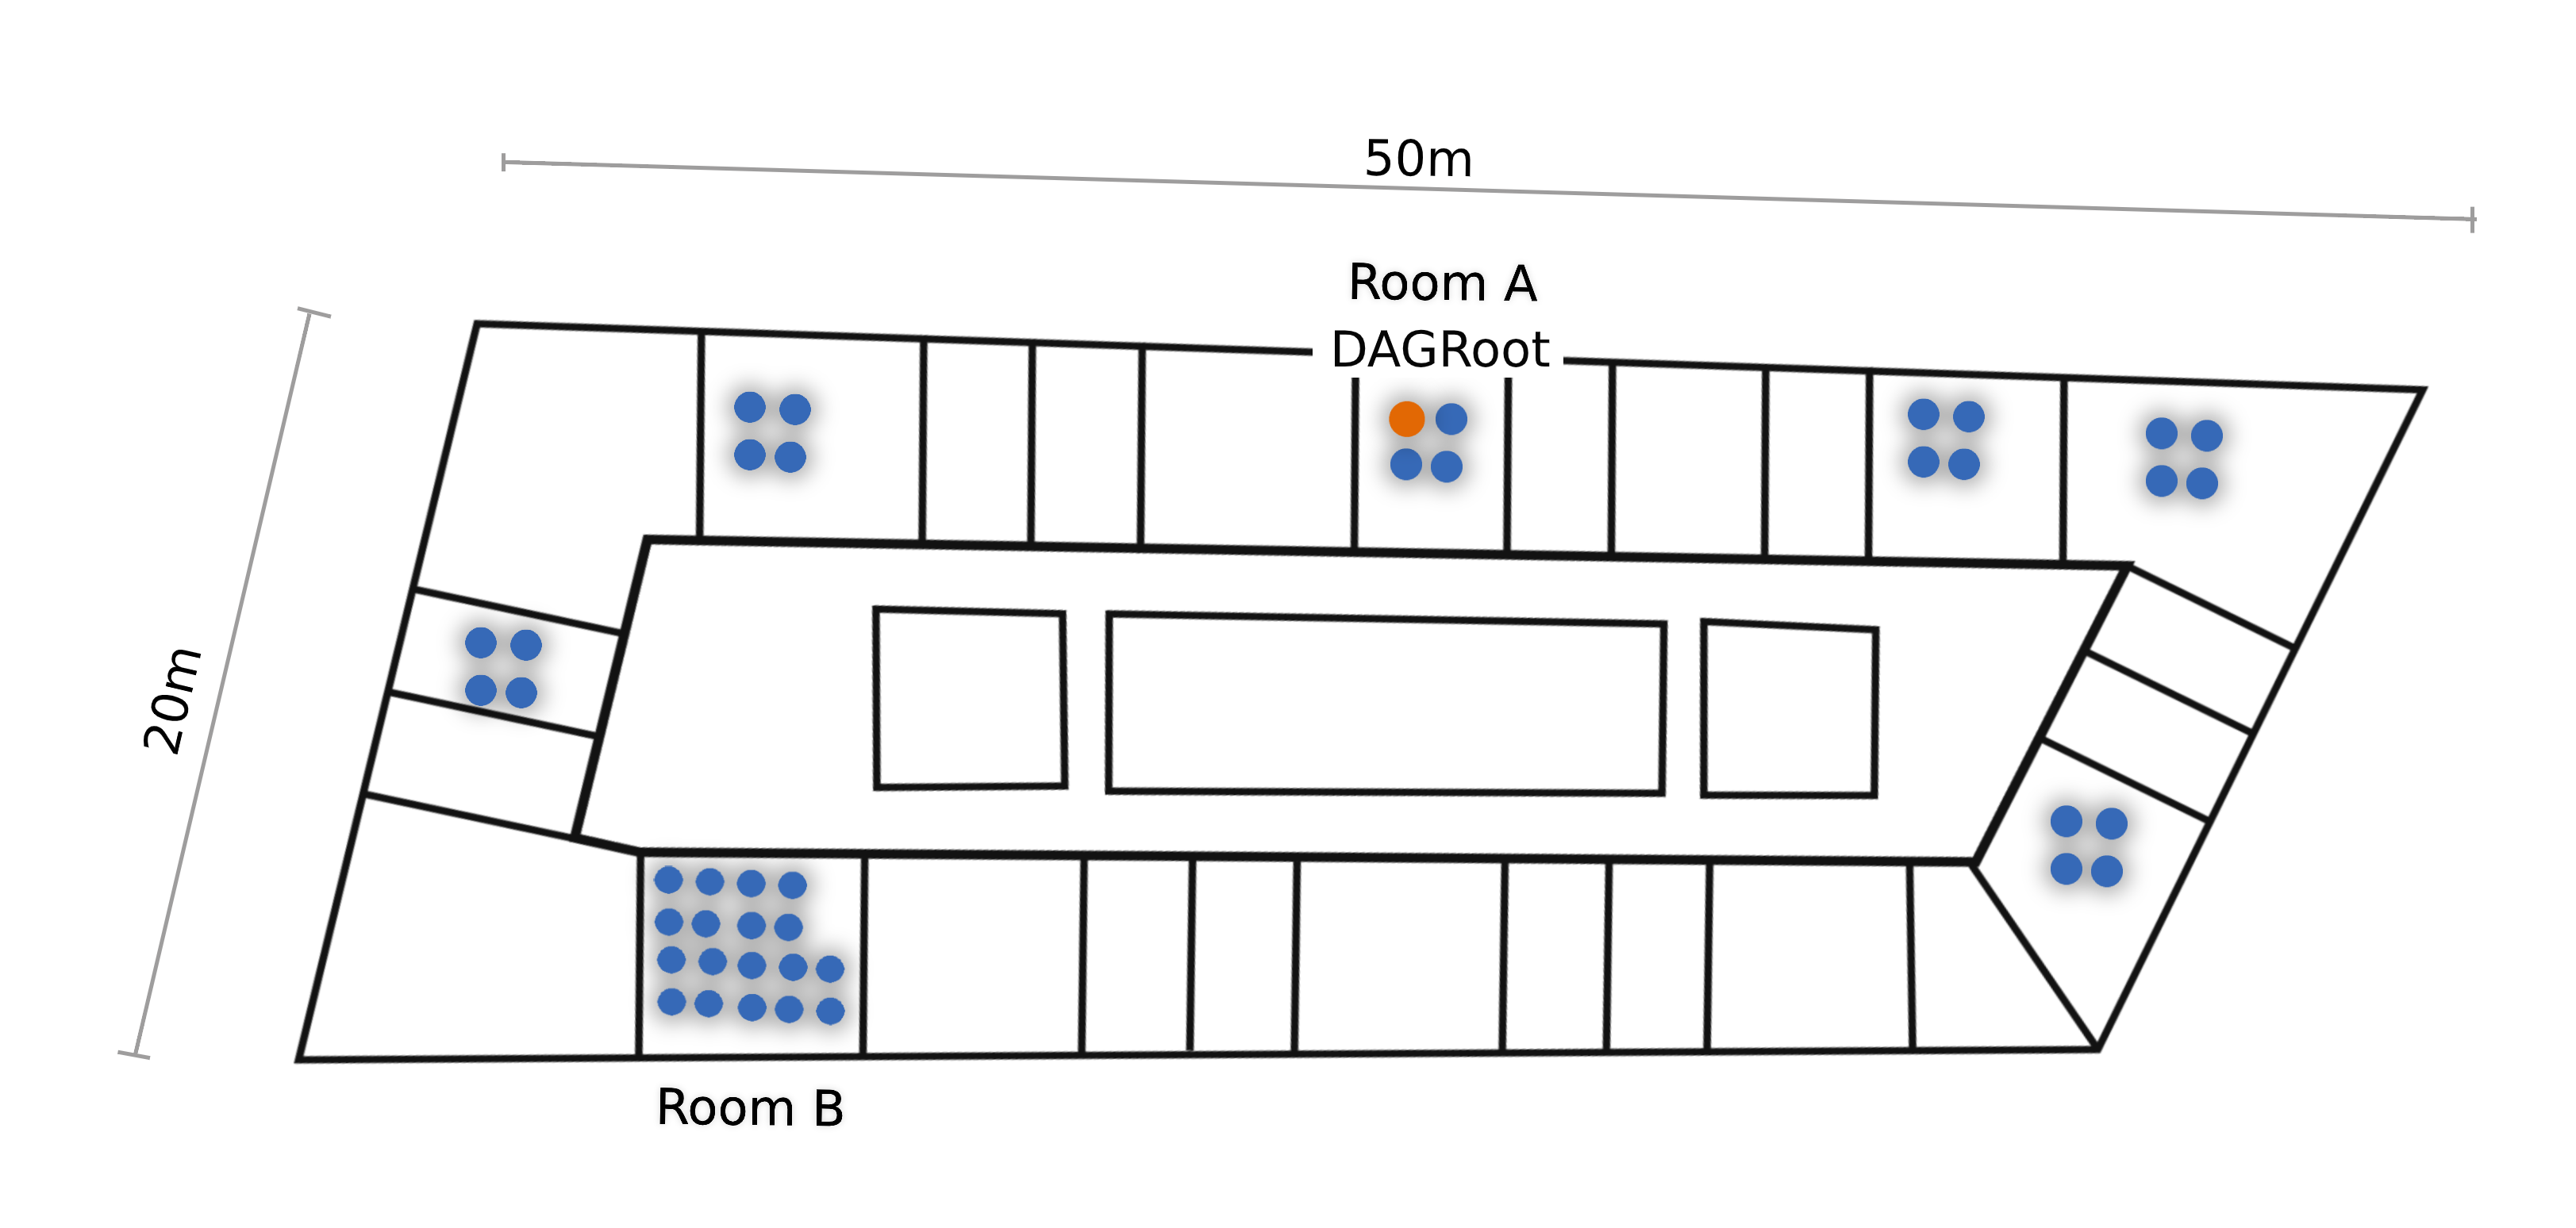
\includegraphics[width=0.90\columnwidth]{building_motes}
	\caption{Floorplan of the deployment.}
    \label{fig:floorplan}
\end{figure}

%==============================================================================
\section{A PHY-layer Agile Extension of OpenWSN}
\label{sec:openwsn}

% intro to 6TiSCH

In efforts to enable industrial-grade low power wireless networking, the IETF has standardized the set of protocol composing what is now known as the IPv6 over the TSCH mode of IEEE802.15.4e, otherwise known as 6TiSCH \cite{vilajosana21ietf}.
The 6tiSCH protocol stack is based on IEEE802.15.4 as its PHY and TSCH mode of IEEE802.15.4e as its MAC layer.
Multi-hop capability is supported at the routing layer via the IPv6 routing protocol for Lower-Power and Lossy Networks (RPL). 
Furthermore, 6LoWPAN is a adaptation layer is defined enabling the interfacing between the routing layer and the specific operations of the MAC layer such as neighbor discovery, registration, ranking, and maintenance operations that impact how routes are calculated. 

% intro to OpenWSN

The 6TiSCH protocol stack has been ported to two main reference architectures: OpenWSN and Contiki-NG. 
Since this work seeks to benefor from the multi-PHY capability of OpenMote-B as explained in section \ref{sec:opentested}, OpenWSN has been selected as the reference architecture for this experiment since it has already been maintained for several boards, including OpenMote-B. 
OpenWSN is an RTOS that allows protocol layers and applications to run side by side on top of a real-time task scheduler implemented based on the interrupt service routine of the micro-processor.
Before the start of this research, OpenWSN was maintained for IEEE802.15.4 O-QPSK 2.4 GHZ radio. 
While a driver was available for the At86rf215 radio to pursue the indoor and outdoor range testing in \cite{munoz18evaluationa} and \cite{munoz18overview}, two challenges were still unmet: 
1) IEEE802.15.4e time-slot templates were not derived for the range of modulations to be tested in this experiment.  Therefore, if the 6TiSCH stack is to run on different modulations, OpenWSN needs to offer multi-slot-template support.
2) OpenWSN has operated based on a single radio-driver only (the CC2538 driver for \oqpsk) . Therefore, if the 6TiSCH stack is to run on different modulations, OpenWSN needs to offer multi-driver support.

% goal: multiple PHY layer
To overcome those challenges, an agile PHY layer needs to be designed for OpenWSN such that any the selected radio option at the physical layer and time-slot template at the MAC layer can change while the rest of the 6TiSCH stack remains intact. 
To this end, three modulations were selected for the experiment: \fsk, \ofdm, and \oqpsk, each representing the extremes of IEEE802.15.4g modulations as longest range, highest bit-rate, and least power consuming, respectively \cite{sotokmscale}
However, instead of simply hard-coding the radio and MAC parameters in the OpenWSN stack to use the new driver and the respective time-slot, a future-proof "parameterized " approach is needed such tat researchers or engineers may adapt the PHY layer freely by simply supplying their slot-templates and radio-drivers as parameters to the RTOS. 

% OpenWSN Extension
\lorem

% result: footprint

\lorem

%==============================================================================
\section{Methodology}
\label{sec:methodology}

% repeating 3 times

\lorem

% duration of one experiment

\lorem

% gathering data, publishing raw results, etc.

\lorem

% KPIs

\lorem

% running the experiments

\lorem

%==============================================================================
\section{Experimental Results}
\label{sec:results}

\lorem

%------------------------------------------------------------------------------
\subsection{Network Formation}
\label{sec:network_formation}

% why is it important, define

\lorem

% worst case from a contention point of view

\lorem

% results

\lorem Fig.~\ref{fig:time_firstpacket_cdf}

\begin{figure}
	\centering
	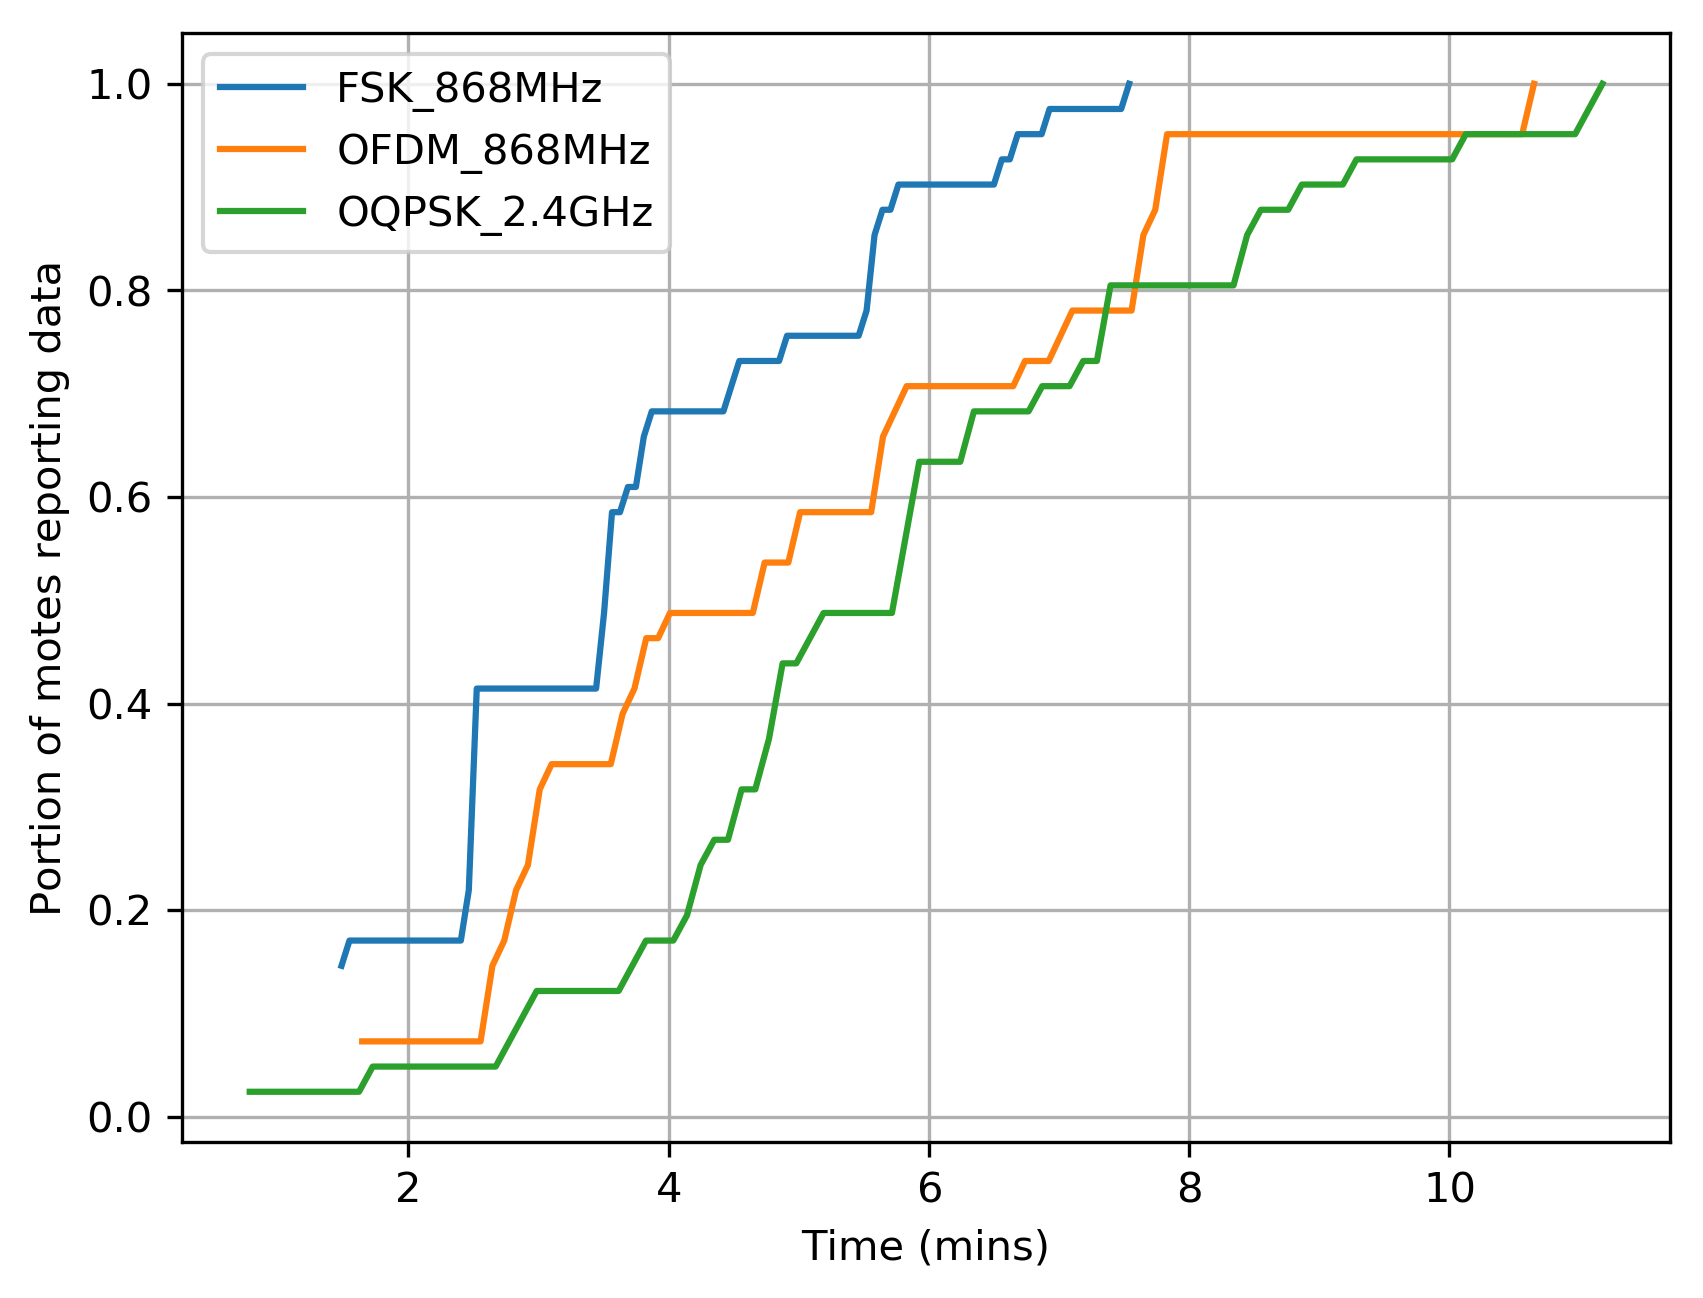
\includegraphics[width=0.90\columnwidth]{time_firstpacket_cdf}
	\caption{Time to First Packet CDF.}
    \label{fig:time_firstpacket_cdf}
\end{figure}

% settling time, steady-state   

\begin{figure}
	\centering
	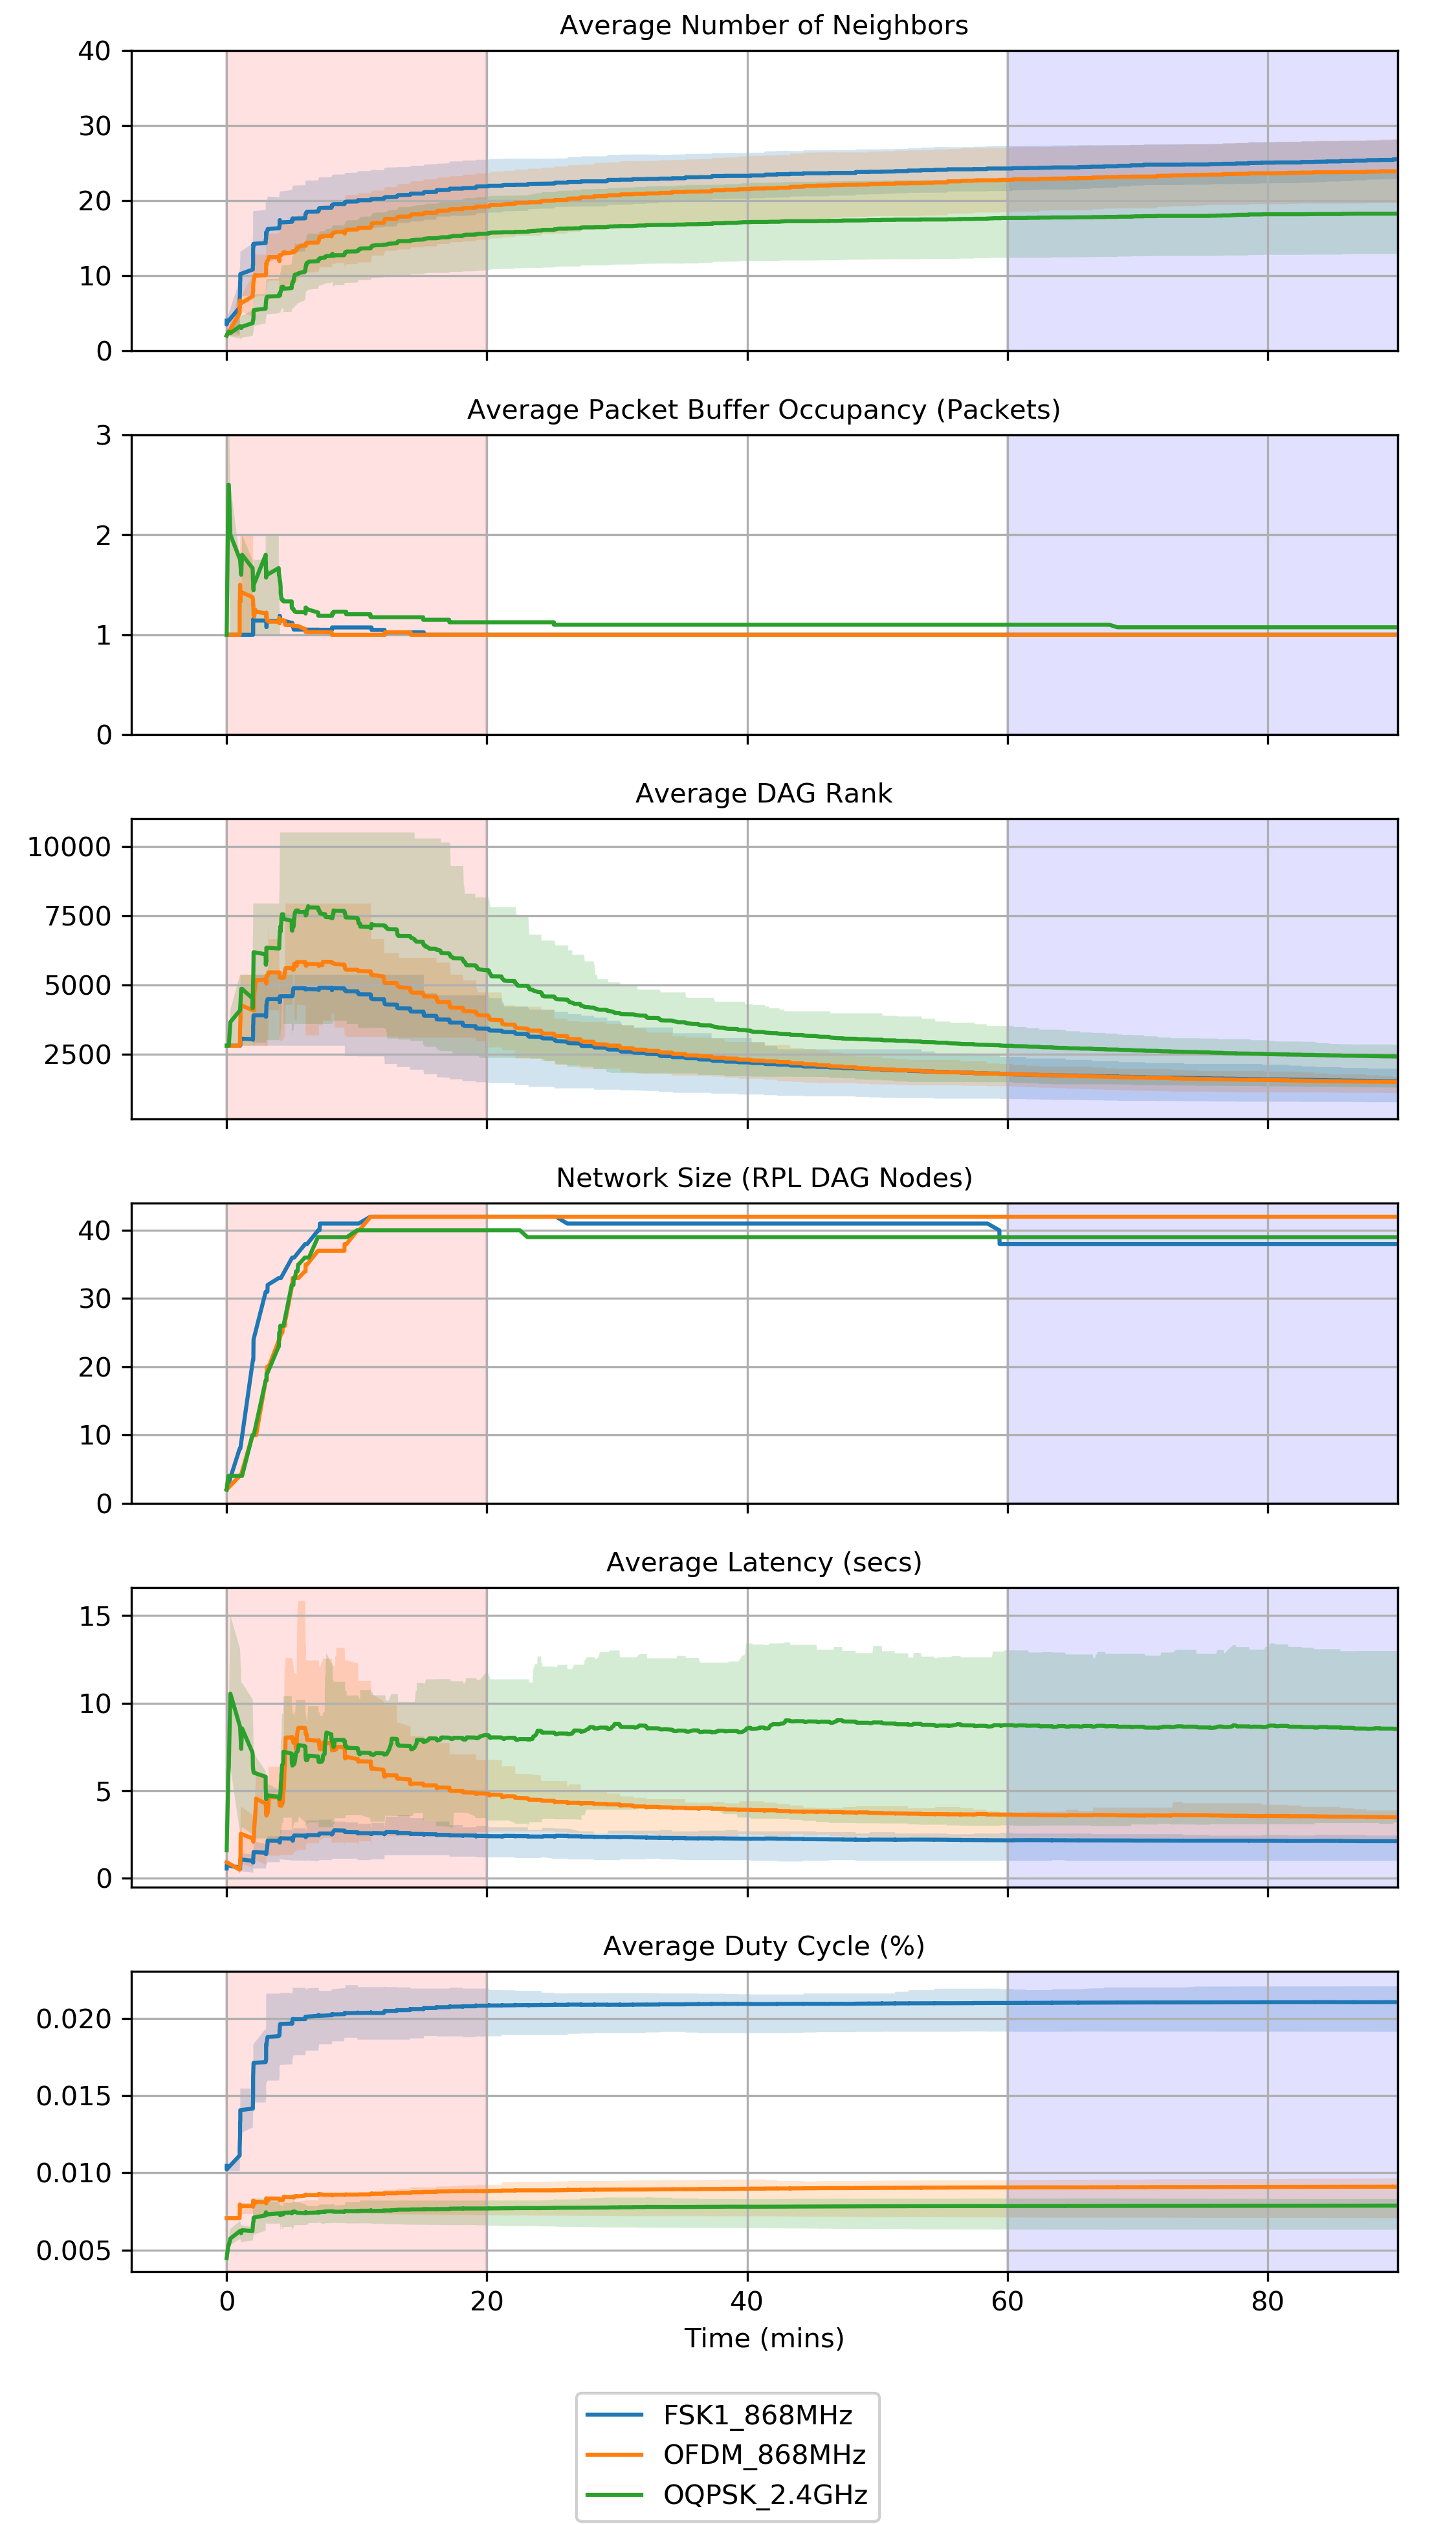
\includegraphics[width=0.90\columnwidth]{aggregate_plot_reliability}
	\caption{6TiSCH reliability performance under each radio setting in the three stages of network formation: 1) discovery and formation phase (red highlight),and 2) steady-state phase (blue highlight). Shaded curves represent the majority of the distribution (interquartile range)}
    \label{fig:aggregate_plot_reliability}
\end{figure}


%------------------------------------------------------------------------------
\subsection{End-to-End Reliability}
\label{sec:reliability}
% why is it important, and how is it measured? 
% Packet loss on shared cells. 
% Long range lead to more neighbors which leads to discovery of better neighbors closer to the root. 

% The negative side is that requires more active and strict rule for accepting neighbors, otherwise it would lead to a neighbor table buffer overflow, specially in dense networks

% Short range can cause more packet loss due to lower link budget if propagation is challenging. 


\begin{table}
 \caption {Steady-state end-to-end PDR values} \label{tab:pdr_table} 
 \begin{center}
 \begin{tabular}{||c c c c||} 
 \hline
 Radio Setting & Average & Median & Stdev \\ [0.5ex] 
 \hline\hline
 \fsk & 100\% & 100\% & 0 \\ 
 \hline
 \ofdm & 99,9521\% & 100\% & 0.302 \\
 \hline
 \oqpsk & 100\% & 100\% & 0 \\
 \hline

\end{tabular}
\end{center}
\end{table}

% plot churn in bar chart or individual charts.

\begin{figure}
	\centering
	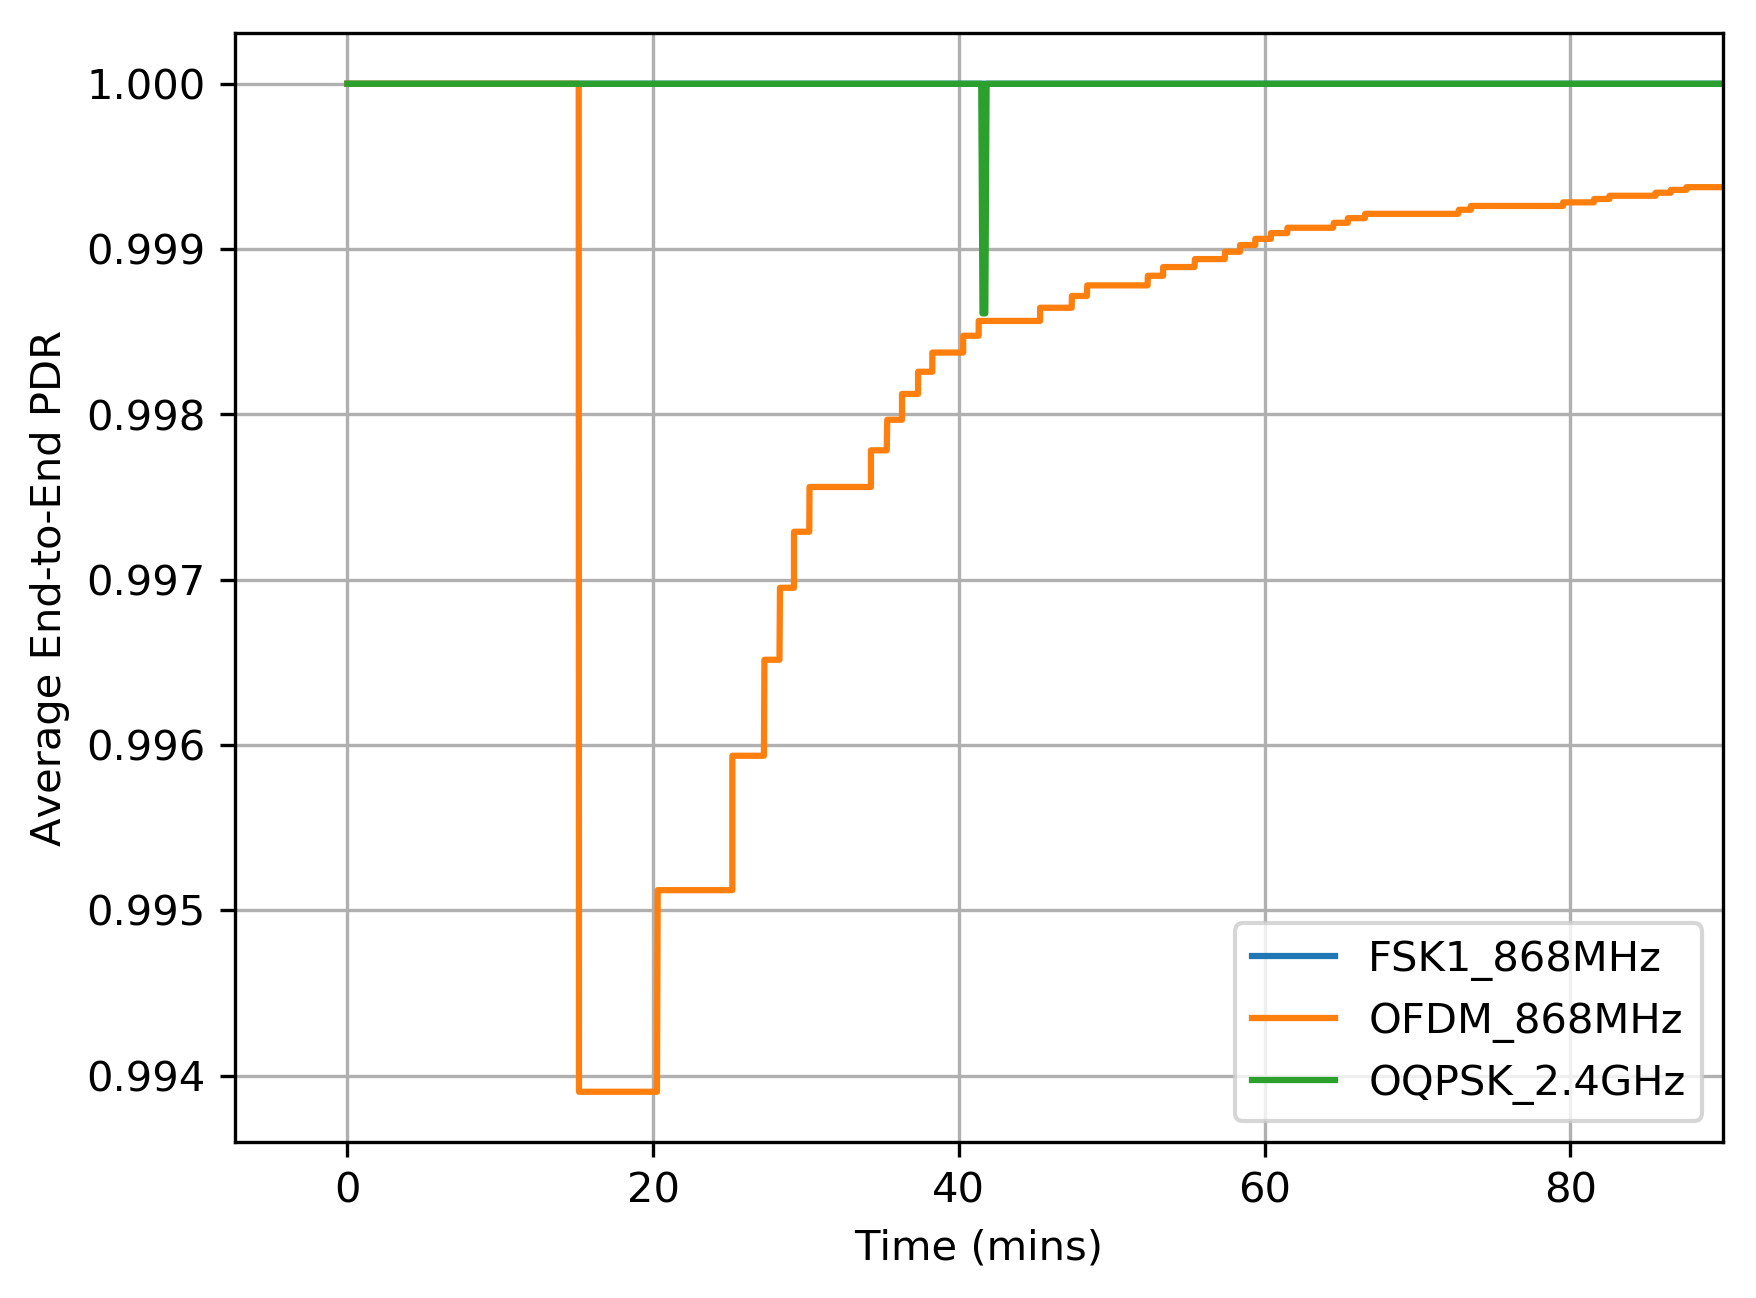
\includegraphics[width=0.9\columnwidth]{avg_pdr_plot.png}
	\caption{Average end-to-end PDR. }
    \label{fig:avg_pdr_plot}
\end{figure} 

%------------------------------------------------------------------------------
\subsection{End-to-End Latency}
\label{sec:latency}

% why is this important? information recency, alarms, logging of critical events for the reactive or preemptive measures.
% higher link budget lead to discovery of more neighbors which leads less hops and less end to end latency.

% shorter range not only suffer from more hops but also more re-transmissions.

\begin{figure}
	\centering
	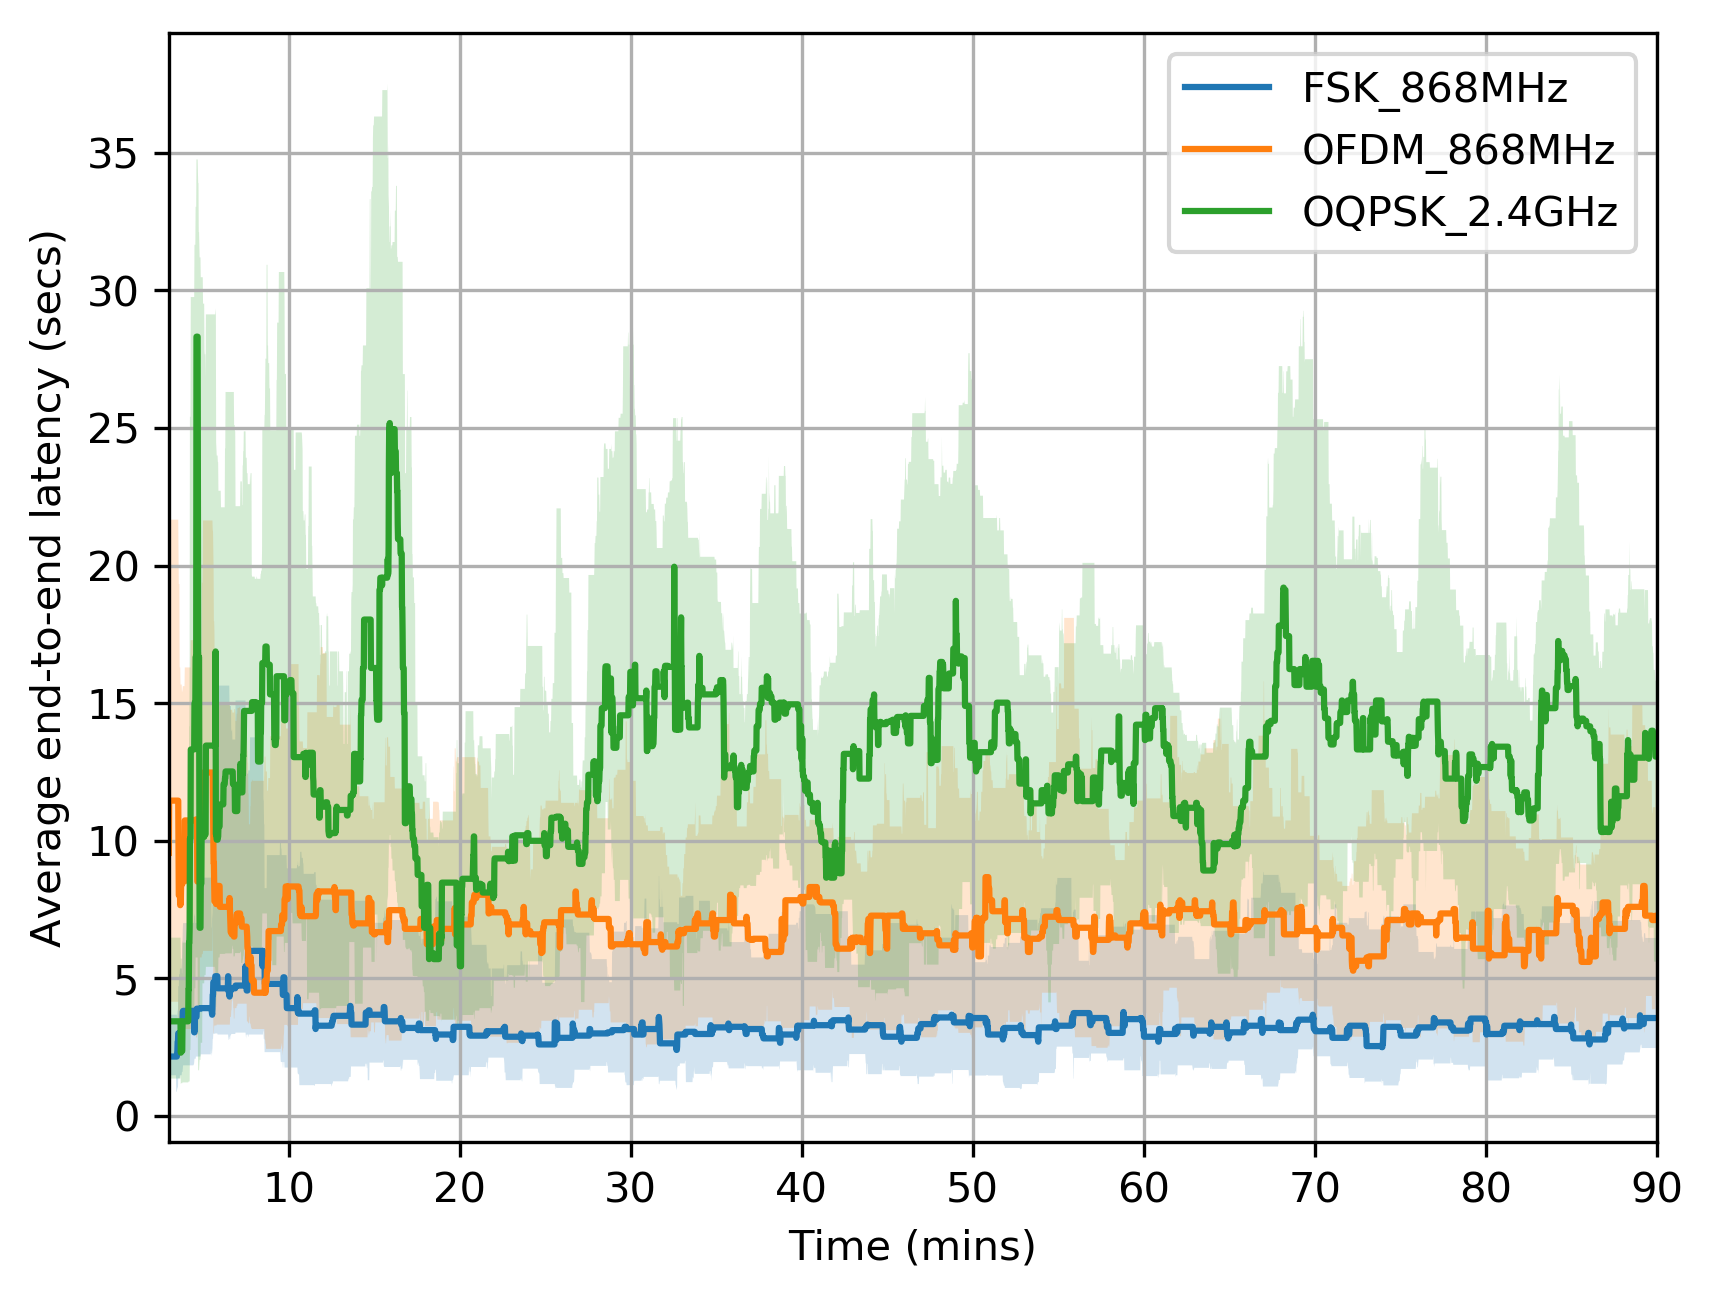
\includegraphics[width=0.90\columnwidth]{avg_latency_plot}
	\caption{Average end-to-end latency. Shaded curves represent the majority of the distribution - i.e. interquartile range (extracted from Fig. \ref{fig:aggregate_plot_reliability})}
    \label{fig:avg_latency_plot}
\end{figure}

%------------------------------------------------------------------------------
\subsection{Queue Occupancy}
\label{sec:queue}


% why is this important? memory limitations, packet loss simply due to unavailable buffer space. 

% Interestingly enough, it seems that there is an inverse correlation between bit-rate and average packet buffer occupancy as seen in Fig.~\ref{fig:avg_bufferSize_plot}. 

% In this setting, the packet queue buffer is of size 20 entries. 



\begin{figure}
	\centering
	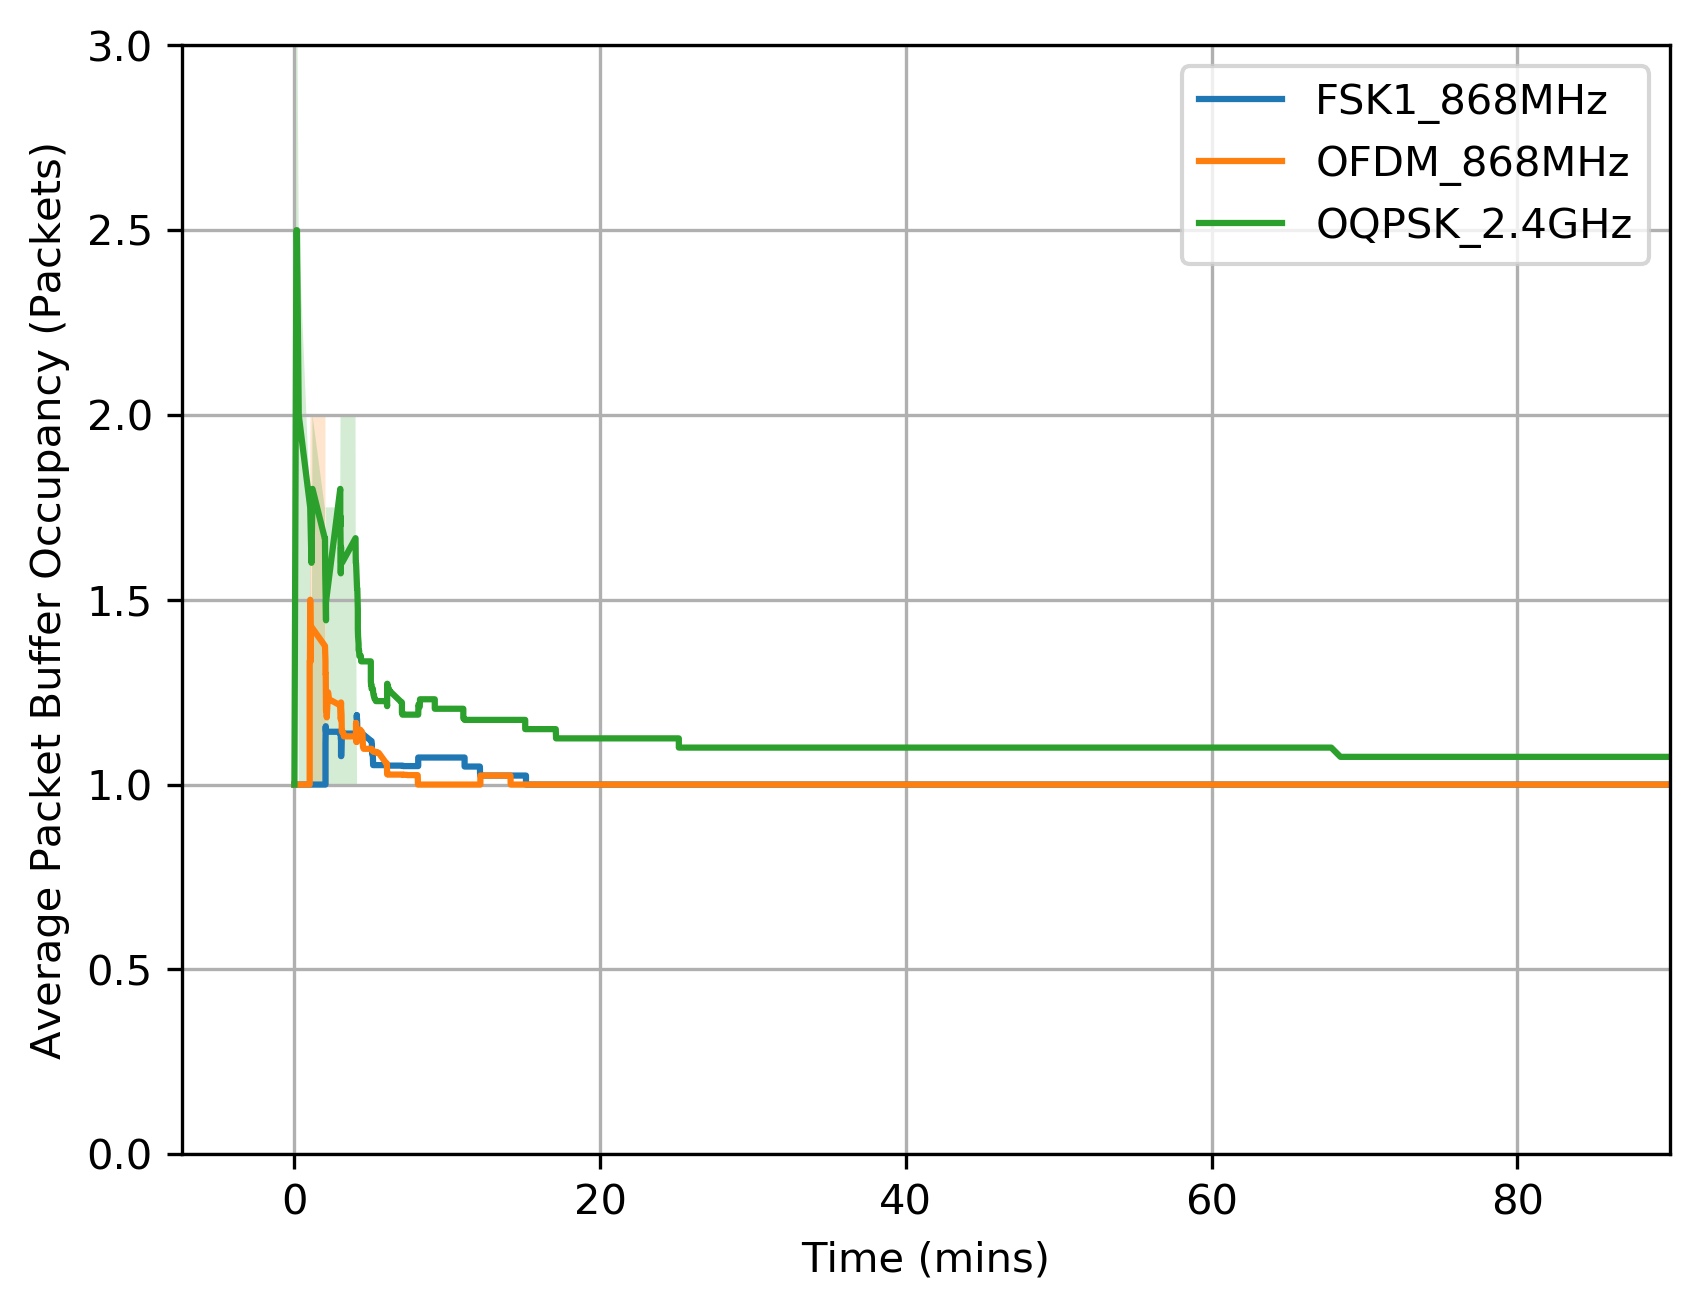
\includegraphics[width=0.90\columnwidth]{avg_bufferSize_plot}
	\caption{Average queue occupancy (extracted from Fig. \ref{fig:aggregate_plot_reliability})}
    \label{fig:avg_bufferSize_plot}
\end{figure}

%------------------------------------------------------------------------------
\subsection{Battery Lifetime}
\label{sec:battery_lifetime}


% why is this important? essential opex. OpEx presents a huge constraint and could lead to impractical deployment if batteries have to change too often (thesis reference)
\begin{figure}
	\centering
	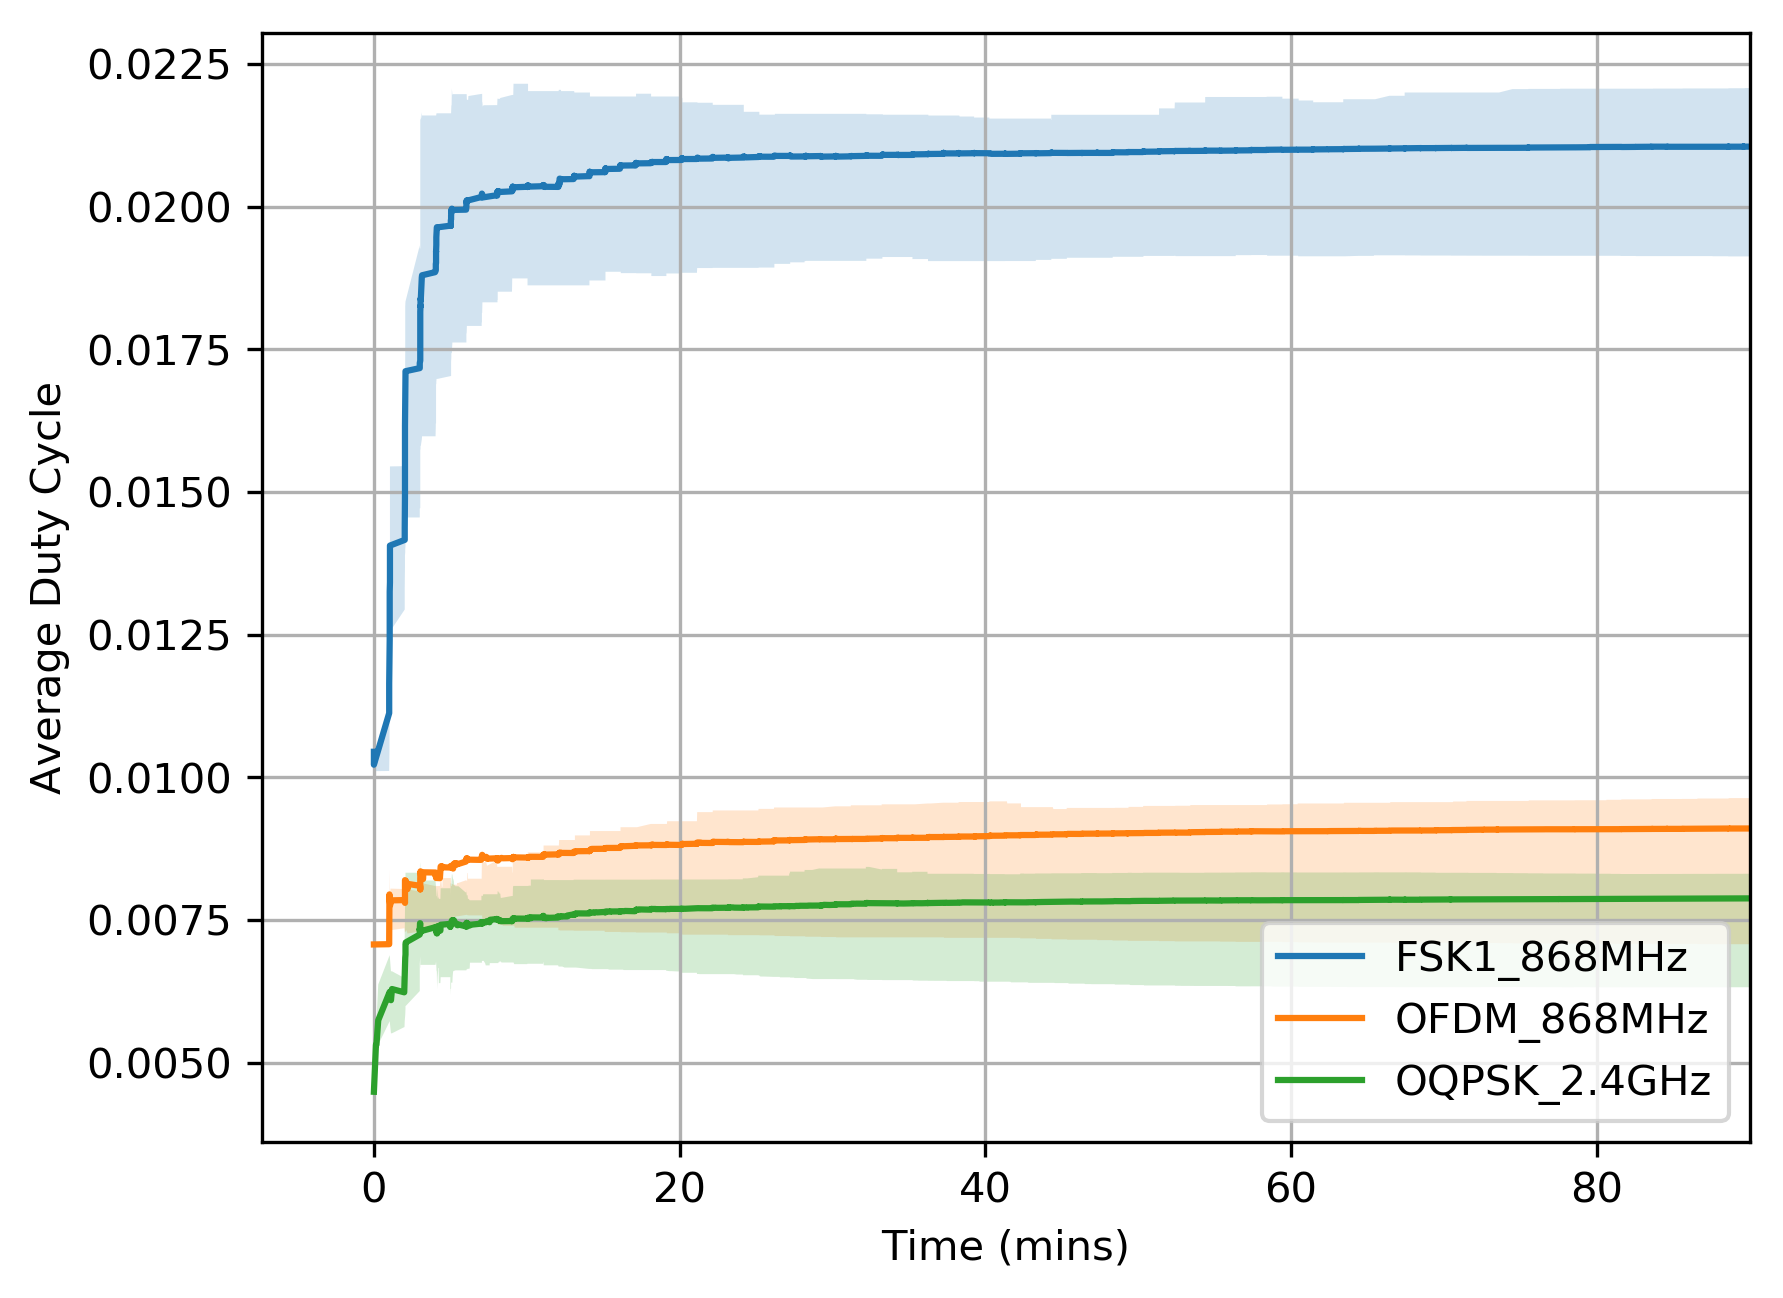
\includegraphics[width=0.90\columnwidth]{avg_avg_dutyCycle_plot}
	\caption{Average duty cycle.Shaded curves represent the majority of the distribution - i.e. interquartile range. (extracted from Fig. \ref{fig:aggregate_plot_reliability})}
    \label{fig:avg_avg_dutyCycle_plot}
\end{figure}

%------------------------------------------------------------------------------
\subsection{Cumulative Comparison of the Results}
\label{sec:cimulative}



\begin{figure}
	\centering
	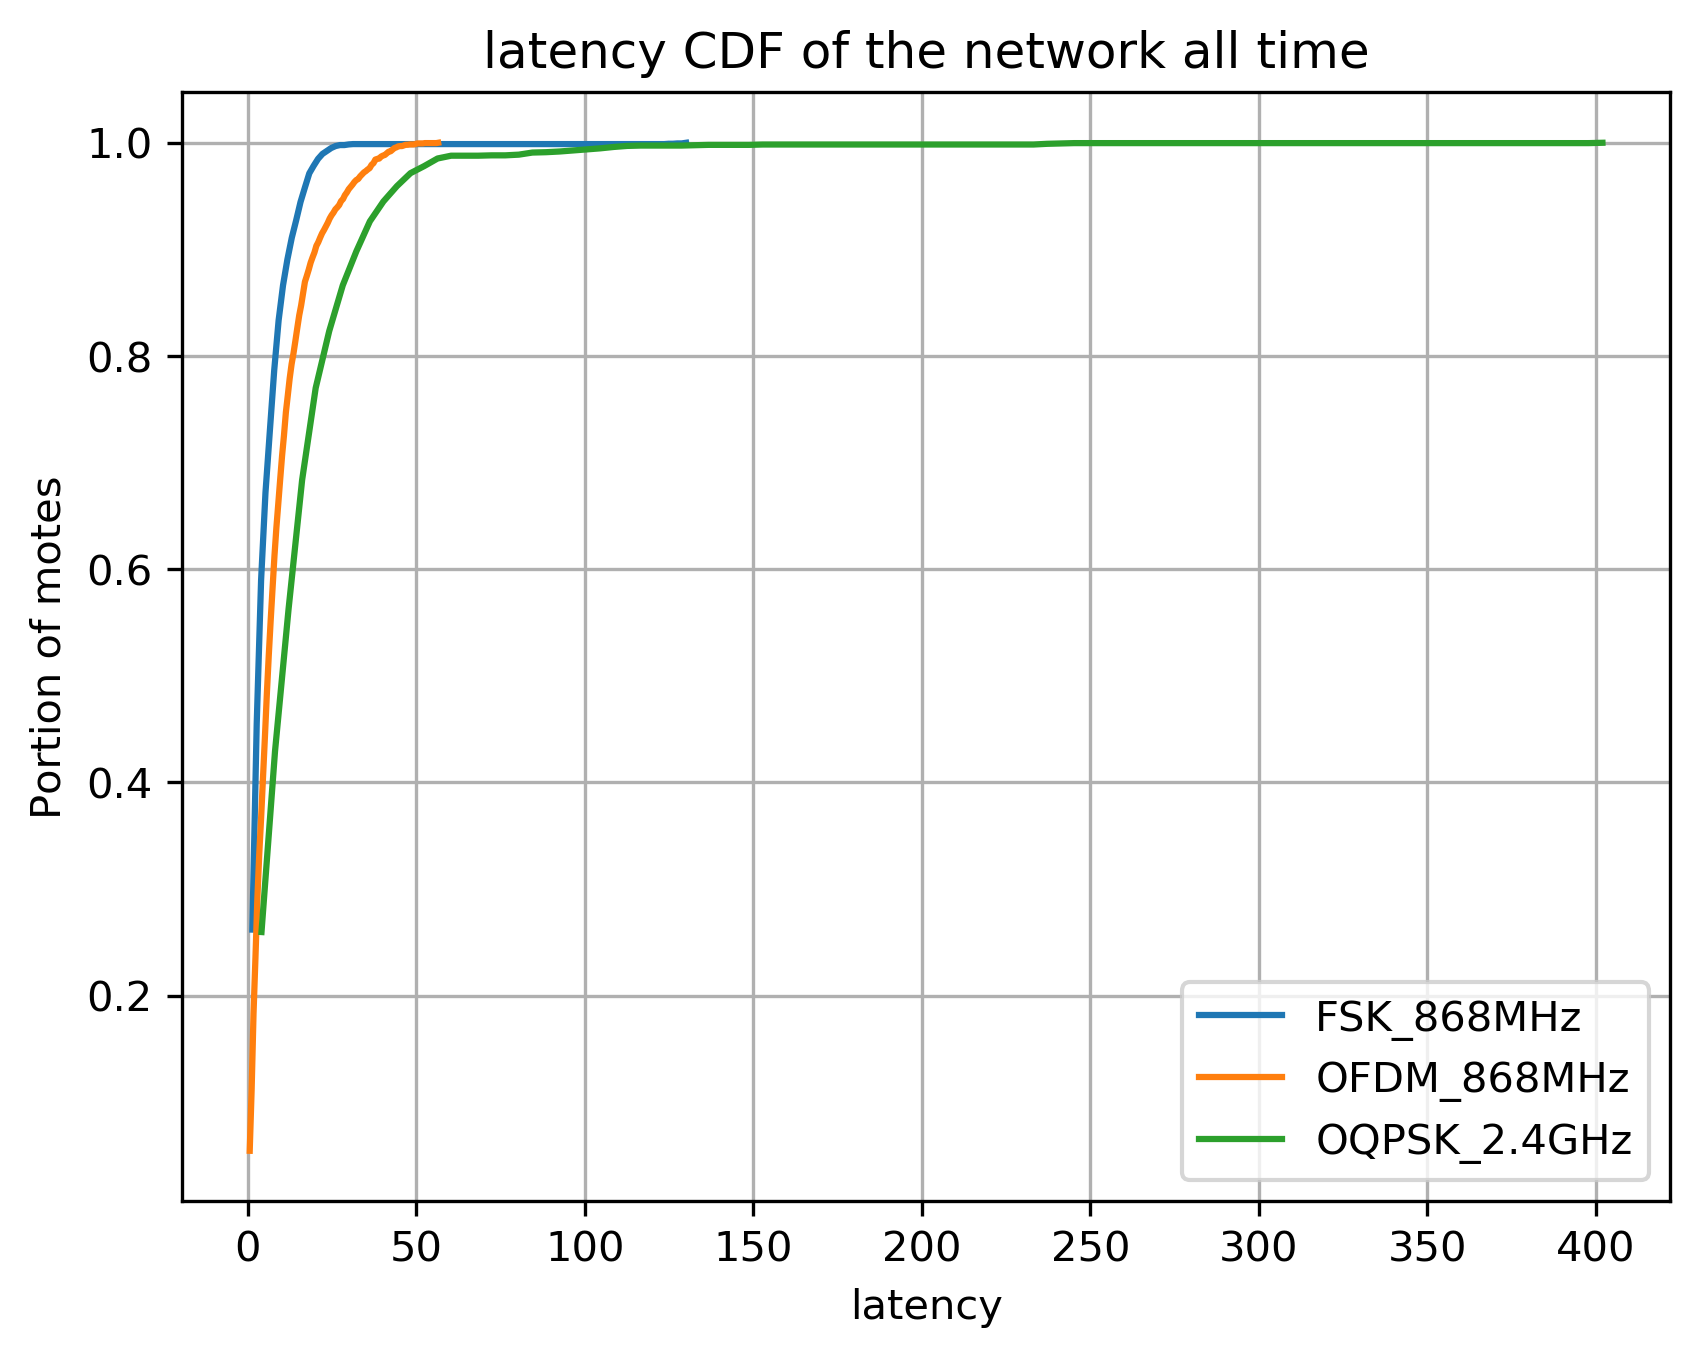
\includegraphics[width=0.90\columnwidth]{latency_cdf_plot_full}
	\caption{CDF of latency in the network} 
    \label{fig:latency_cdf_plot_full}
\end{figure}

\begin{figure}
	\centering
	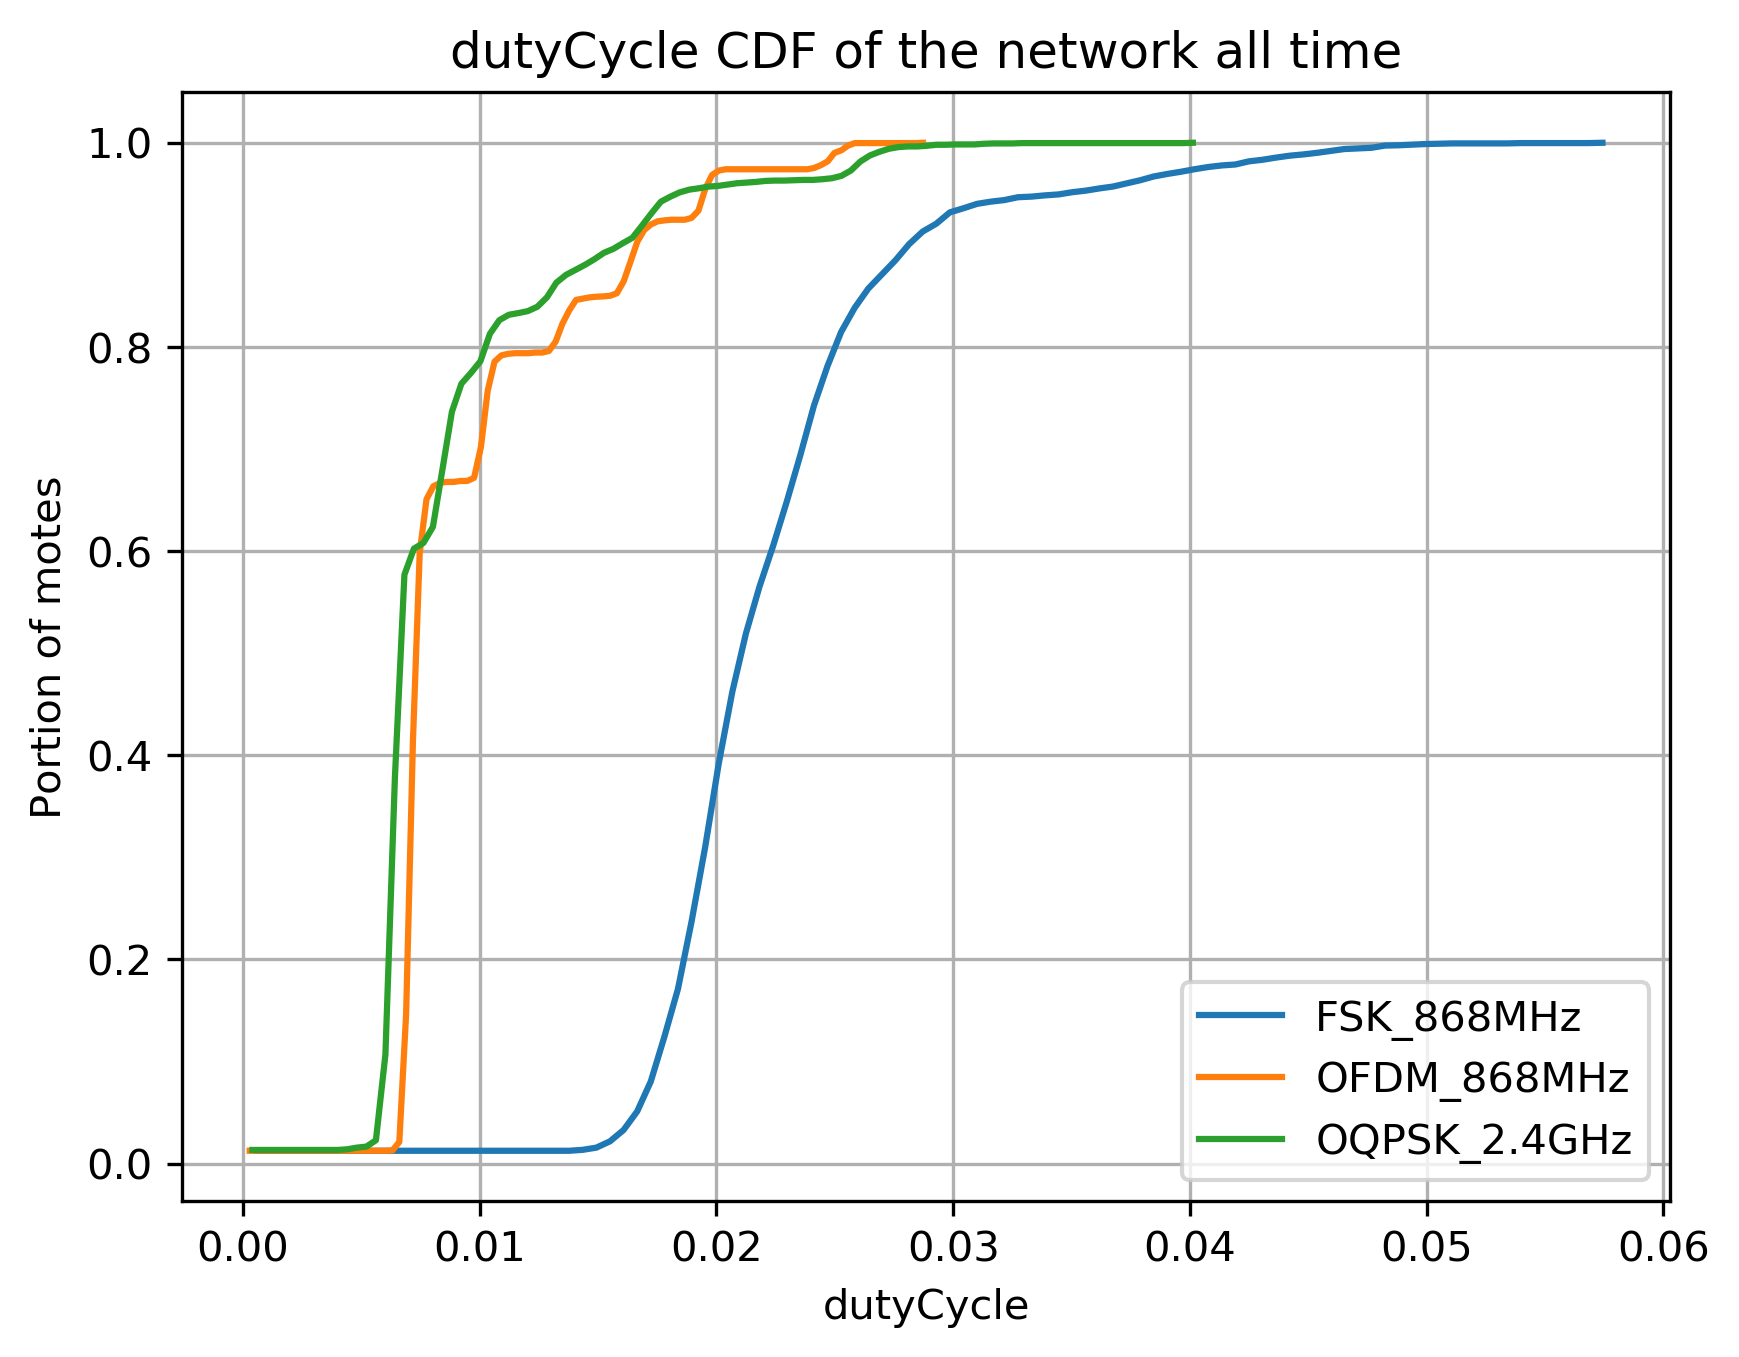
\includegraphics[width=0.90\columnwidth]{dutyCycle_cdf_plot_full}
	\caption{CDF of radio duty cycle in the network} 
    \label{fig:dutyCycle_cdf_plot_full}
\end{figure}

\begin{figure}
	\centering
	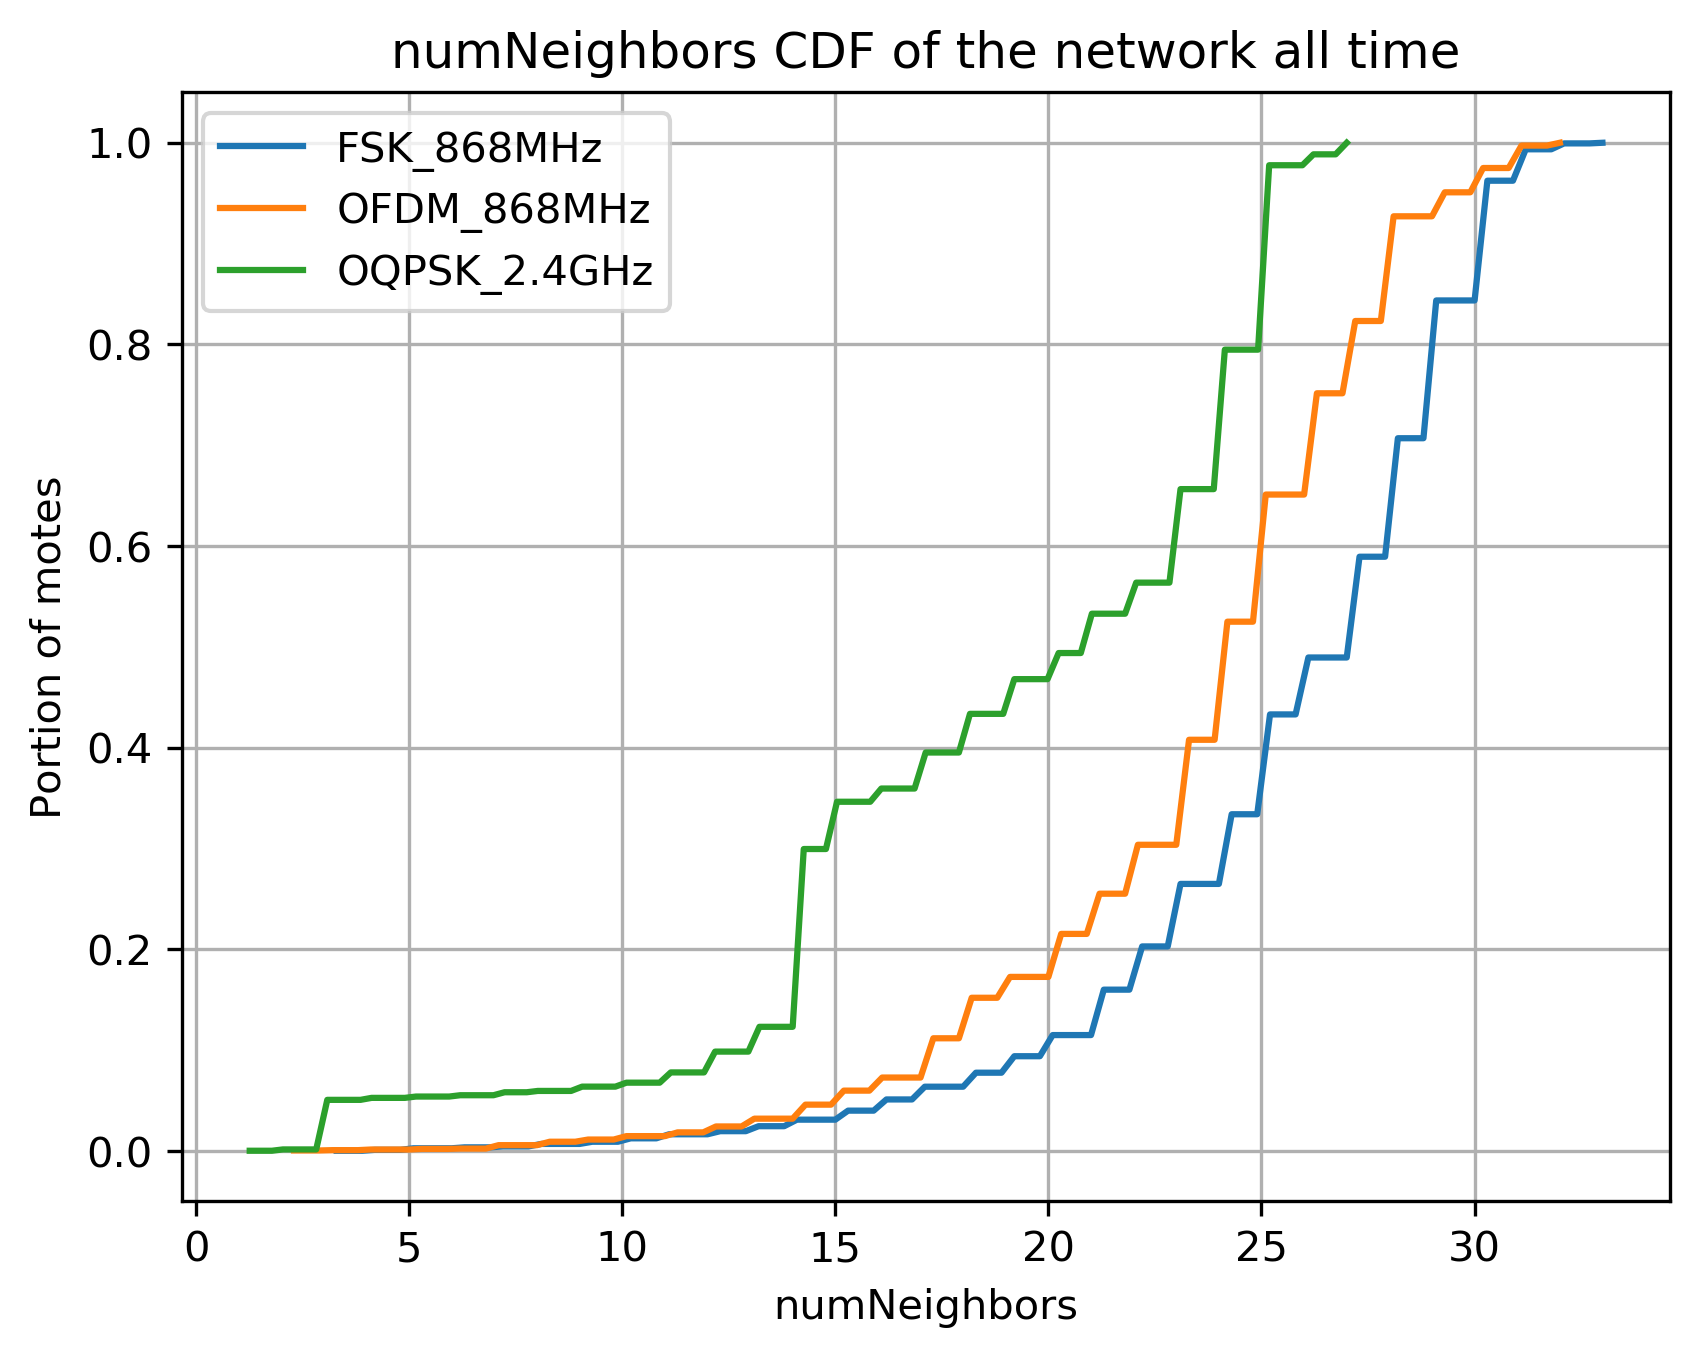
\includegraphics[width=0.90\columnwidth]{numNeighbors_cdf_plot_full}
	\caption{CDF of number of neighbors in the network} 
    \label{fig:numNeighbors_cdf_plot_full}
\end{figure}

\begin{figure}
	\centering
	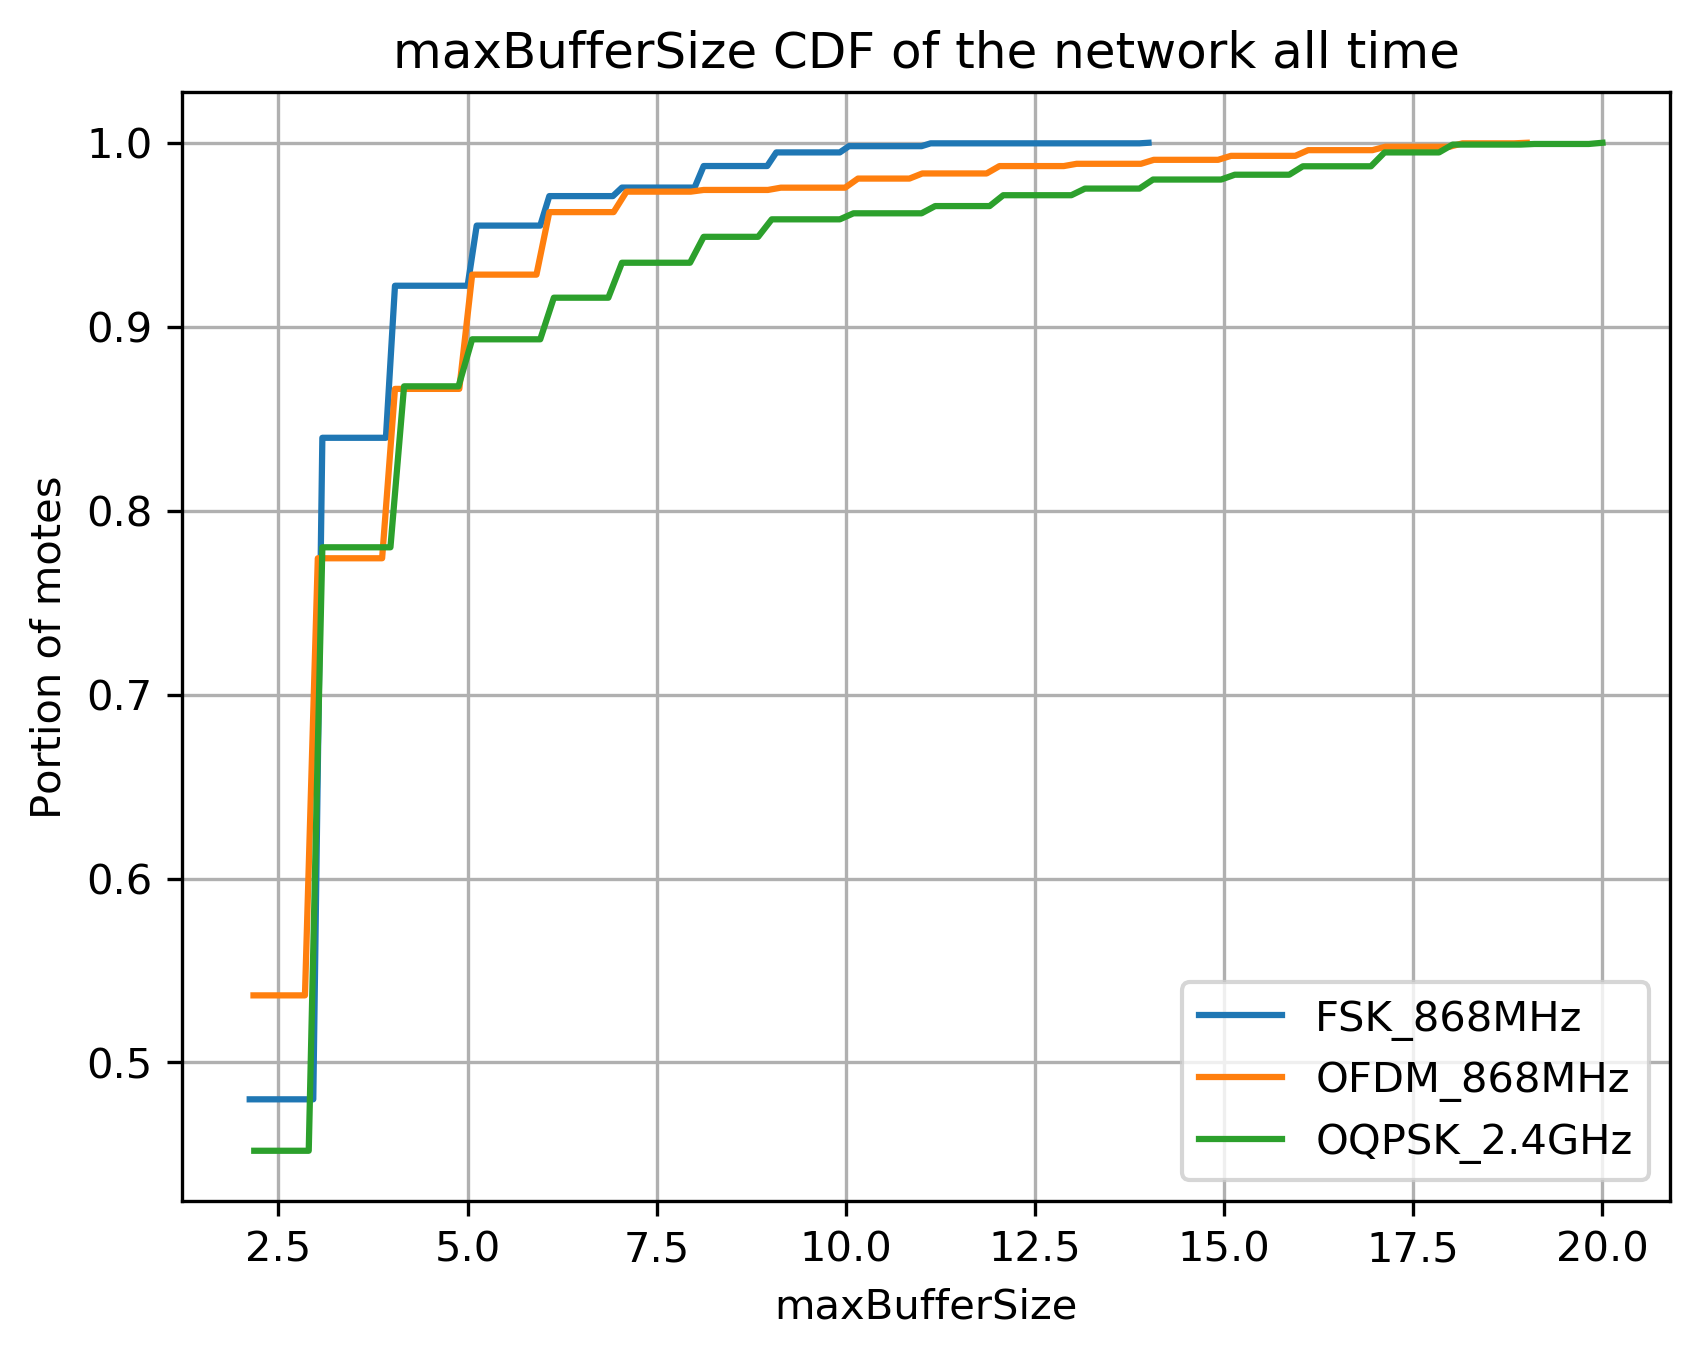
\includegraphics[width=0.90\columnwidth]{maxBufferSize_cdf_plot_full}
	\caption{CDF of max packet buffer occupancy in the network} 
    \label{fig:maxBufferSize_cdf_plot_full}
\end{figure}
\begin{figure}
	\centering
	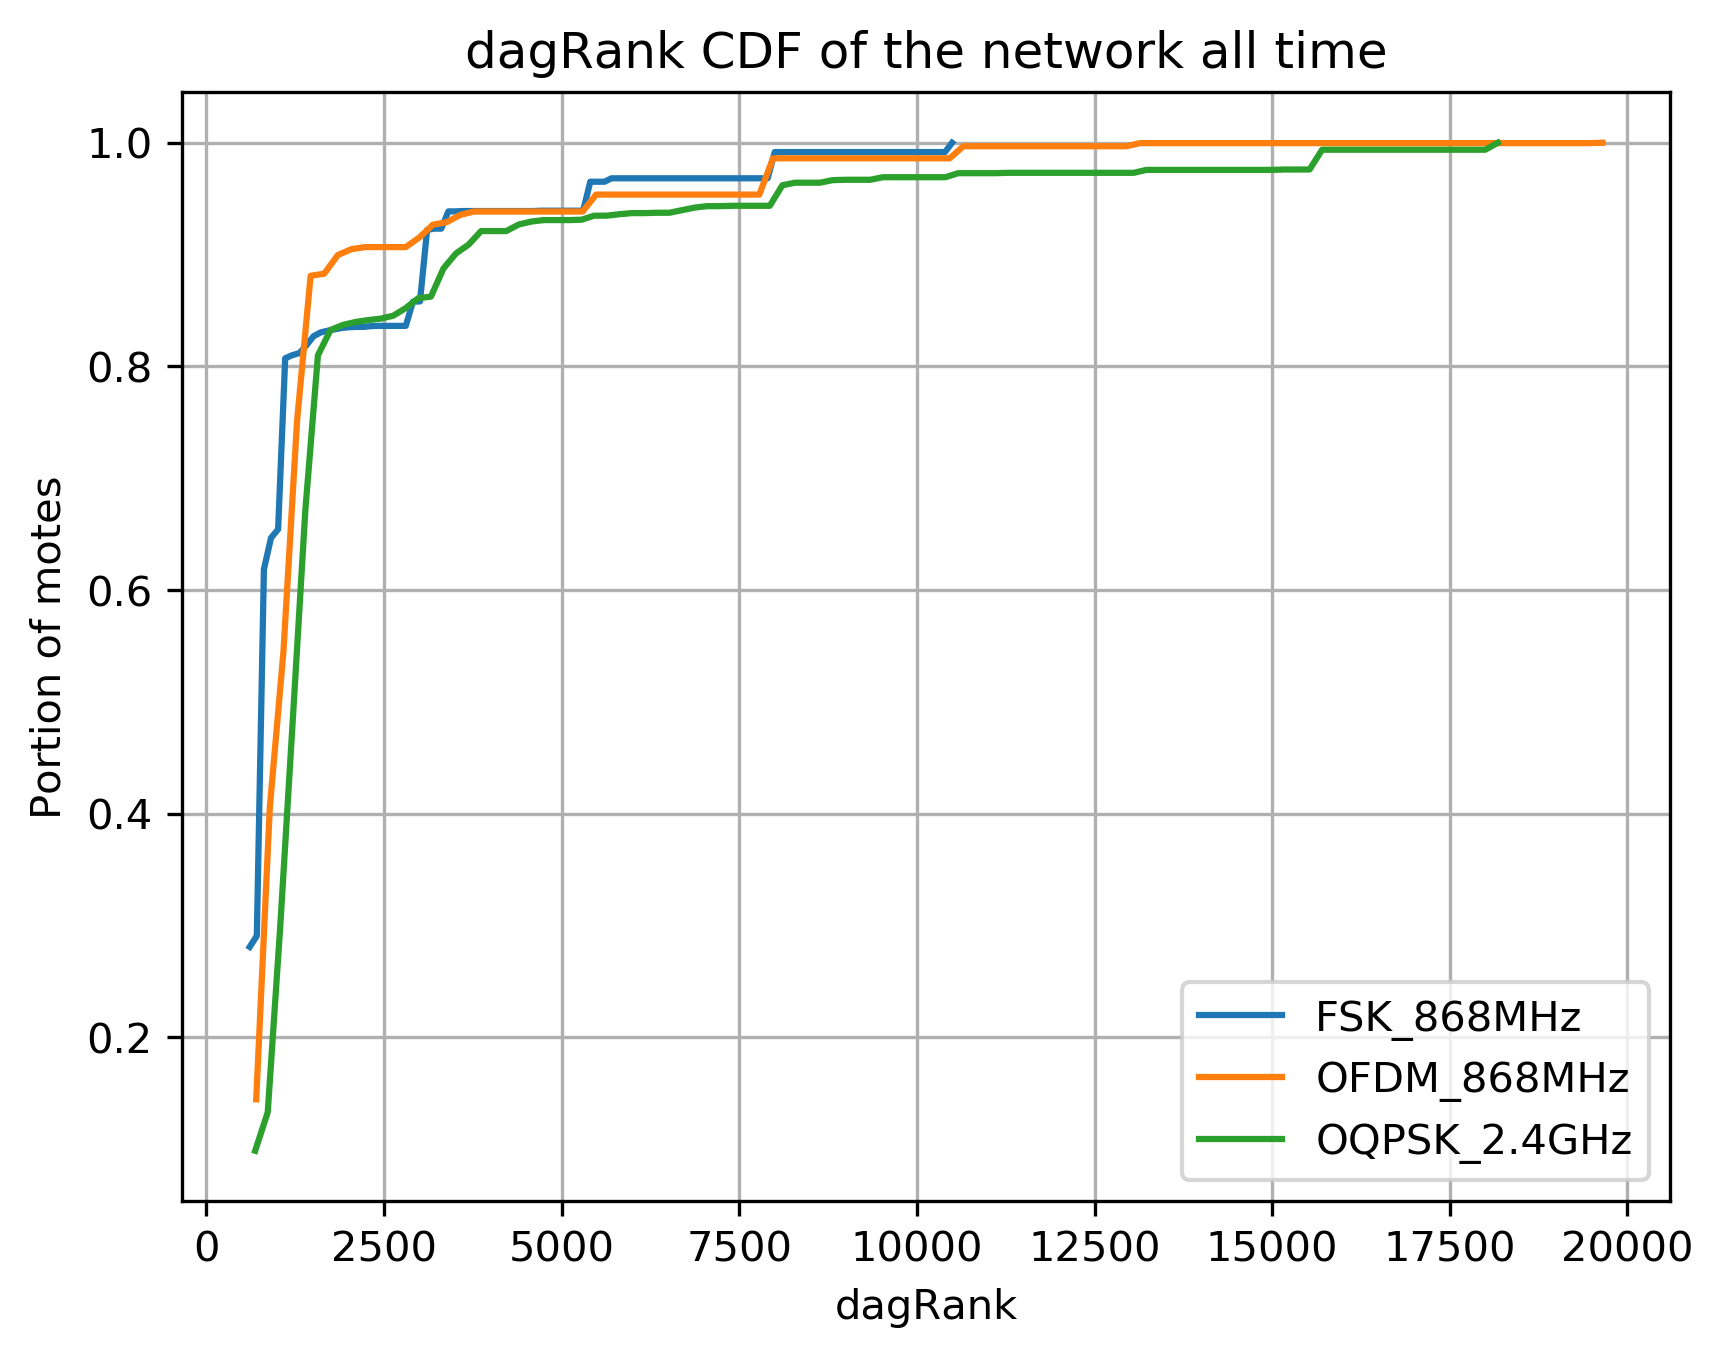
\includegraphics[width=0.90\columnwidth]{dagRank_cdf_plot_full}
	\caption{CDF of DAG Rank in the network} 
    \label{fig:{dagRank_cdf_plot_full}}
\end{figure}




\mina{mention the exact tx power levels you are using}
\begin{table*}[t]
 \caption {Battery Life - assuming 2 AA batteries with total 3V and 4.2 wh capacity} \label{tab:energy_table} 
 \begin{center}
\begin{tabular}{lllllllll}
      & Total DC & Tx DC (measured) &  \begin{tabular}[c]{@{}l@{}}RX DC\\ (estimated)\end{tabular} & \begin{tabular}[c]{@{}l@{}}Tx Current \\ (mA)\end{tabular} & \begin{tabular}[c]{@{}l@{}}Rx Current\\  (mA)\end{tabular} & \begin{tabular}[c]{@{}l@{}}Tx Power Consuption \\ (wh)\end{tabular} & \begin{tabular}[c]{@{}l@{}}Rx Power Consumption\\  (wh)\end{tabular} & \begin{tabular}[c]{@{}l@{}}Battery lifetime\\  (days)\end{tabular} \\
\fsk   & 0,02     & 0,00225          & 0,01775                                                     & 62                                                         & 28                                                         & 0,186                                                               & 0,084                                                                & 251,4997                                                           \\
\ofdm  & 0,00875  & 0,000375         & 0,008375                                                    & 62                                                         & 28                                                         & 0,186                                                               & 0,084                                                                & 872,3785                                                           \\
\oqpsk & 0,0077   & 0,0005           & 0,0072                                                      & 24                                                         & 20                                                         & 0,072                                                               & 0,06                                                                 & 2607,892                                                          
\end{tabular}
\end{center}
\end{table*}
%------------------------------------------------------------------------------
\section{Discussion}
\label{sec:discussion}
\begin{table*}[t]
 \caption {6TiSCH performance ranking for each setting} \label{tab:summary}
\begin{tabular}{lllllllll}
      & network fomration speed. & energy & latency & buffer effeciency & pdr &  &  &  \\
\fsk   & 1                        & 3      & 1       & 1                 & 1   &  &  &  \\
\ofdm  & 1                        & 2      & 2       & 1                 & 2   &  &  &  \\
\oqpsk & 3                        & 1      & 3       & 2                 & 1   &  &  & 
\end{tabular}
\end{table*}


%\begin{figure}
%	\centering
%	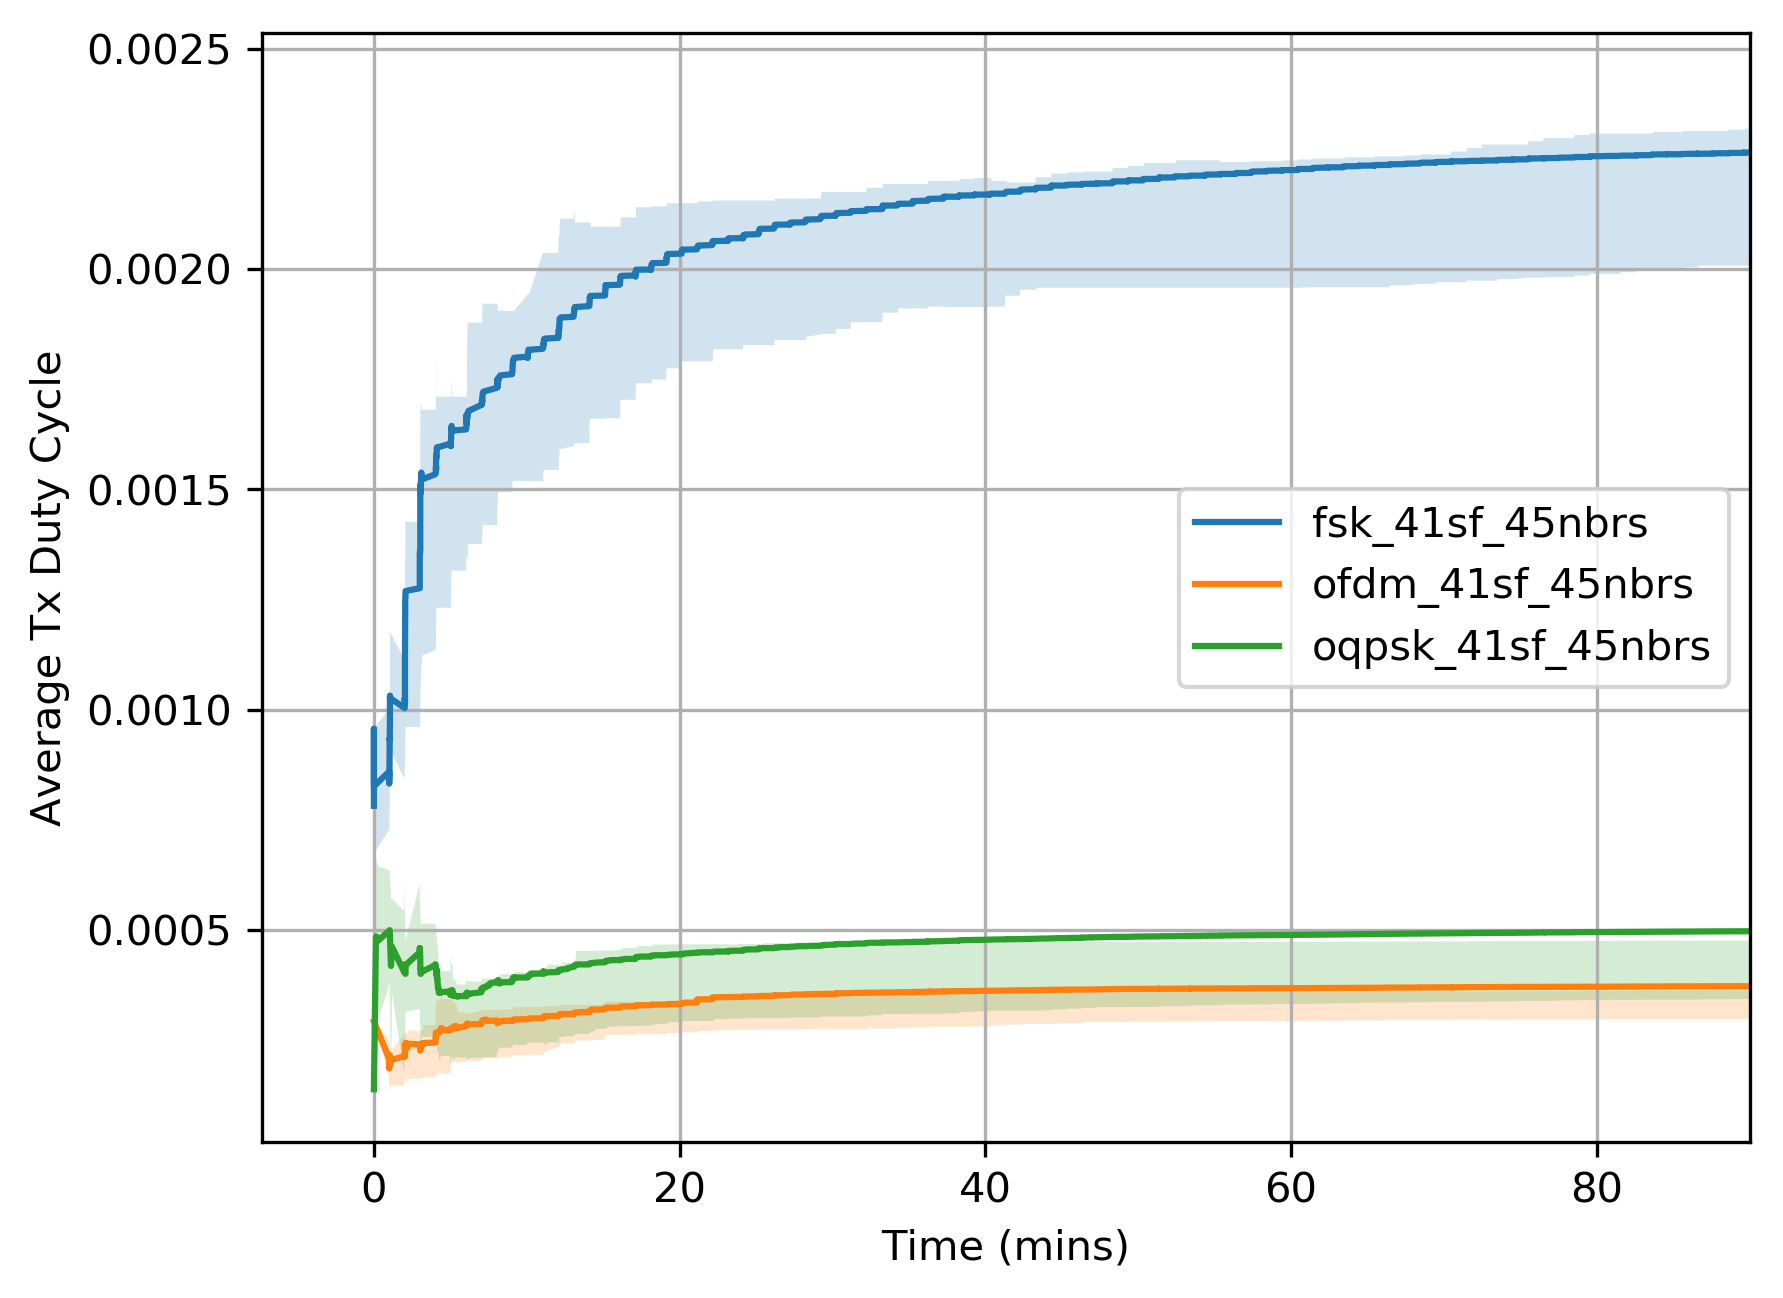
\includegraphics[width=0.90\columnwidth]{avg_avg_dutyCycleTx_plot}
%	\caption{Average transmission duty cycle}
%   \label{fig:avg_avg_dutyCycleTx_plot}
%\end{figure}

%------------------------------------------------------------------------------

\printbibliography

%==============================================================================
\end{document}

%==============================================================================
\section{Summary}

The experiments evaluate the impact of utilization of different radio access technologies at the physical layer of the 6TiSCH stack.
\begin{itemize}
    \item FSK 1 in the subghz band
    \item OFDM 1 MCS3 in the subghz band
    \item OQPSK in the 2.4 GHz band
\end{itemize}

The stack performance is evaluated at a end-to-end looking at  KPIs relevant to an SLA for a critical infrastructure, namely:
\begin{itemize}
    \item Network formation time: defined as CDF of time to first packet from all connected motes within a 30 minute time span.
    \item Reliability: defined in terms of PDR
    \item Quality of Service: defined as traffic latency
    \item Battery lifetime: expected lifetime with a power supply of 2 AA batteries.
    \item Resilience: defined as combination of two metrics: PDR of connected motes and ratio of disconnected motes (i.e. motes that were once connected) after sudden total failure of 10\% of the motes in the network (fixed set). 
\end{itemize}
    
Furthermore, the stack performance on top of each radio is evaluated at system-level for the following scenarios:
\begin{itemize}
    \item Increased traffic demand (by 300\%)
    \item Lower Network size and density (by 50\%)
\end{itemize}

%==============================================================================
\section{Draft outline}

\begin{enumerate}
    \item We explore the performance of the 6TiSCH stack in heterogeneous radio settings and we comment on the following aspects of the stack performance: network formation, reliability, quality of service, and power consumption. We observe the following. \item FSK leads to faster network formation (section \ref{sec:network_formation}). 
    \item However, FSK , as robust as it is, can lead to overall lower end-to-end reliability , which is contrary to the case of OFDM (section \ref{sec:reliability}) 
    \item Despite the lower PDR of the 6TiSCH stack in top of FSK, it shows much more end-to-end stable latency. (section \ref{sec:quality_of_service})
    \item Shorter range radios , even though they consume less energy in principle, they have a side effect as they can lead to the occupancy of the packet memory buffer due to consistent re-transmissions. This could risk reaching buffer overflow as network traffic increases. (section \ref{sec:quality_of_service})
    \item Furthermore, higher reliability of OFDM does not mean higher resilience. 
    Even though OFDM shows 99.6-100\% PDR on average compared to 99.0-99.5\% average PDR for FSK, FSK shows the best resilience in terms of PDR maintenance.  
    FSK result into a higher network degree which risks reaching limits of allocated memory buffers allocated for storage of neighbor information (section \ref{sec:resilience})
    \item Despite the advantages of FSK for end-to-end latency and network formation speed, its power consumption present a significant drawback. Also, despite the higher bitrate of OFDM compared to OQPSK, it ends up consuming similar duty cycles (b/c of re-transmissions?) (section \ref{sec:battery_lifetime})
\end{enumerate}

\begin{figure}
	\centering
	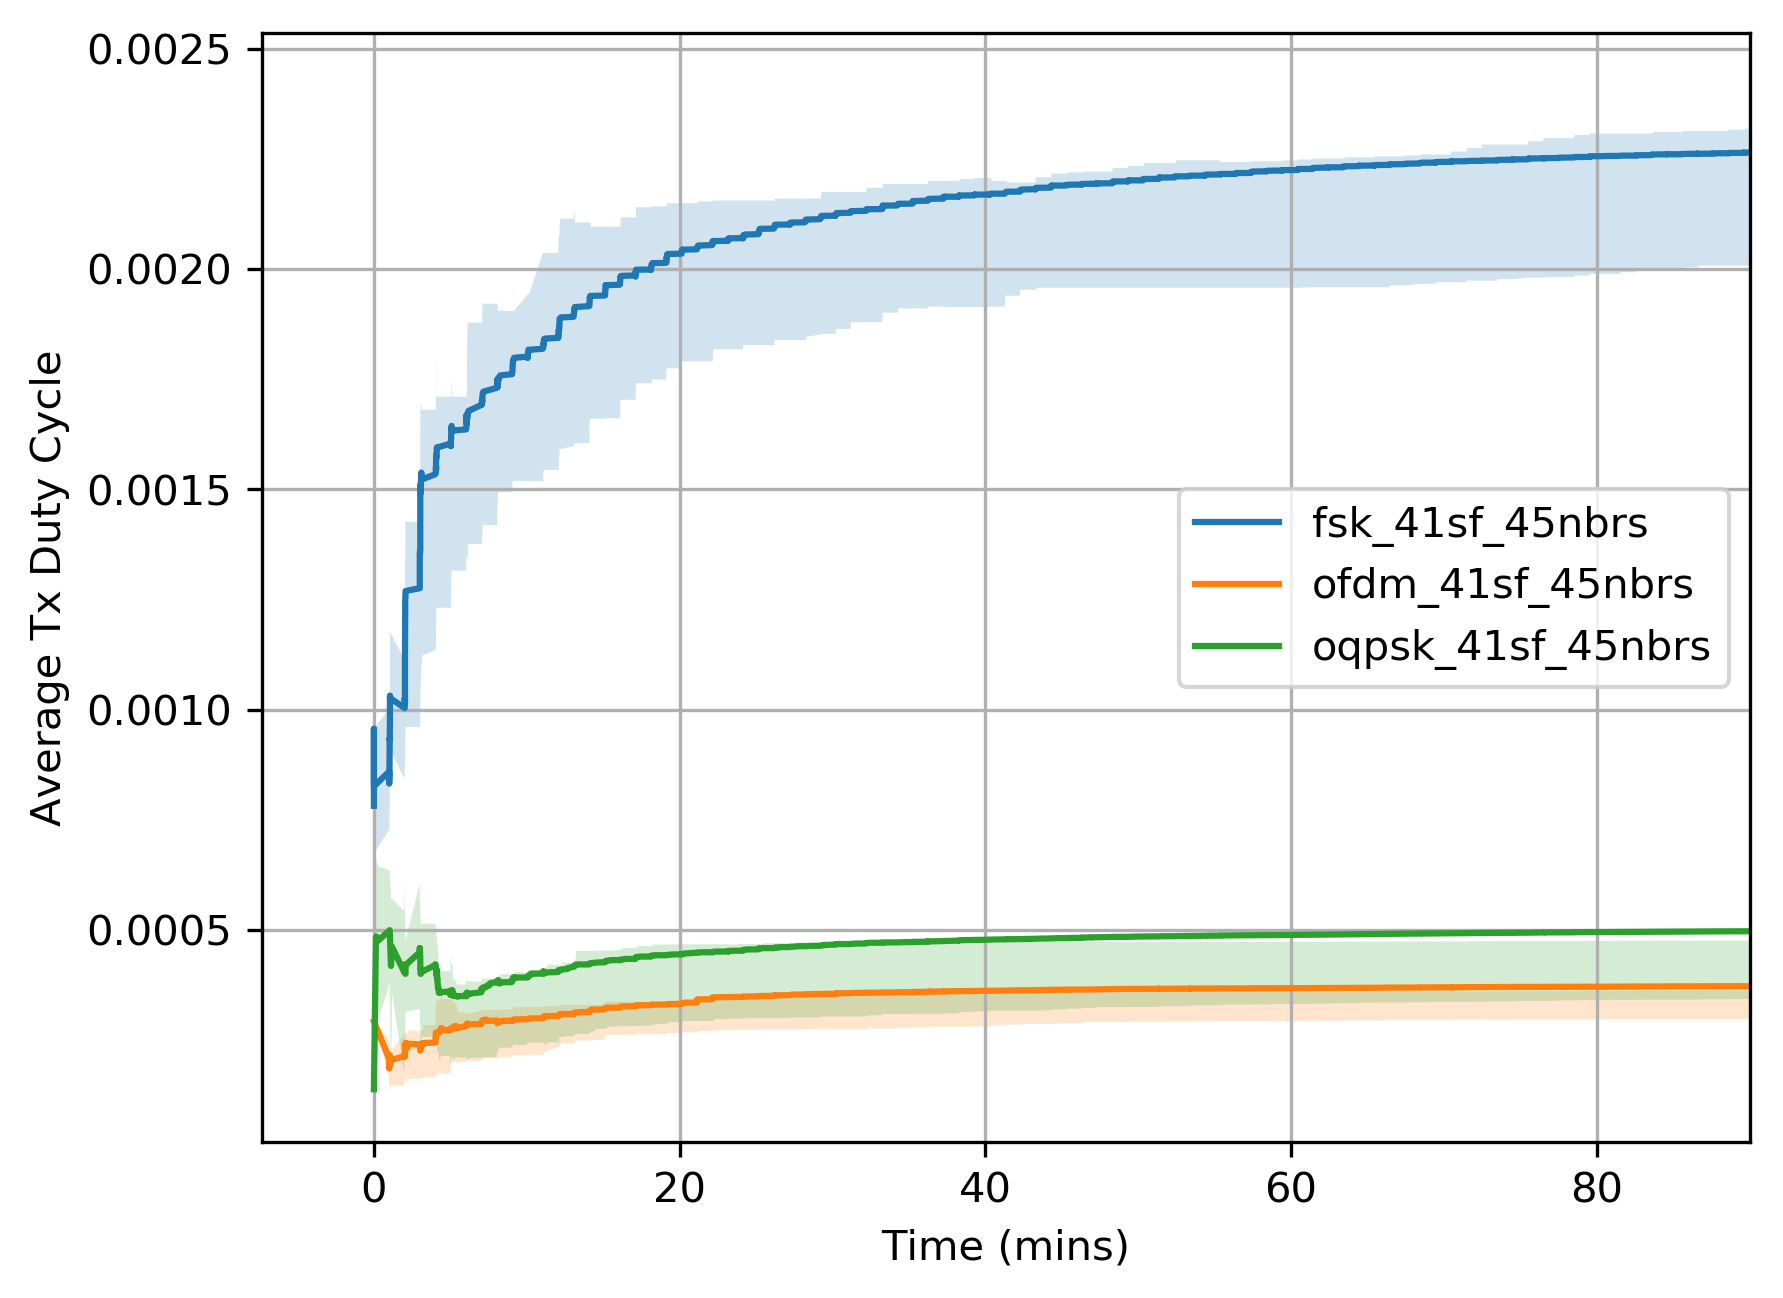
\includegraphics[width=0.90\columnwidth]{avg_avg_dutyCycleTx_plot}
	\caption{Average duty cycle. Shaded curves represent the majority of the distribution (interquartile range).}
    \label{fig:avg_avg_dutyCycleTx_plot}
\end{figure}